
%%%%%%%%%%%%%%% INTRO %%%%%%%%%%%%%%%%%%%%%

IRON: Theoretically, there are three dominant pathways that eddies can effect iron availability. First, during eddy amplification eddy pumping in cyclones (anticylones) can create and upward (downward) flux of iron as isopycnals are domed (depressed). Second, mixed layer modification (see section 3.2) is likely to detrain (entrain) iron rich waters from depth leading to a decrease (increase) in iron avliability in cyclones (anticyclones). Third, Ekman pumping created by the relative motion between surface currents and the wind occurs throughout an eddy's lifetime and should create down-welling (up-welling) in cyclones (anticyclones).

Given the competing mechanisms modifying biogeochemistry within eddies \parencite{McGillicuddyMechanismsPhysicalBiologicalBiogeochemicalInteraction2016} and the fact that net population growth is not always well coupled to division rates \parencite{RohrVariabilitymechanismscontrolling2017,BehrenfeldAnnualcyclesecological2013} it can be problematic to infer depth integrated net primary production exclusively from $[Chl]_{S}'$).

problems associated with infering depth integrated primary productivity from assuming net population growth and division rates are well coupled \parencite{RohrVariabilitymechanismscontrolling2017,BehrenfeldAnnualcyclesecological2013} it is helpful


because net population growth is not always well coupled to division rates \parencite{RohrVariabilitymechanismscontrolling2017,BehrenfeldAnnualcyclesecological2013} it can be problematic to infer primary production exclusively from standing stocks of surface biomass (or $[Chl]_{S}'$).

In order to further constrain the precise biogeochemical response to eddies and understand if observed changes to $[Chl]_{S}'$  reflect population integrated changes in primary production it is helpful to 1) isolate only closed mesoscale structures 2) specifically account for changes in the component rate terms that comprise net population growth (i.e. division rates, loss rates), and 3) consider the entire depth integrated biogeochemical response and structure of the biomass profile.

DIVISION RATES: The bulk effect of bottom-up controls on phytoplankton growth can be directly represented by the population specific division rate ($\mu_\Sigma'$). Anomolous division rates within eddy interiors reveal how the eddies may influence bottom-up controls on phytoplankton population growth.


Variability in $\mu_\Sigma'$ is primarily driven can be understood by variability in the comunity mean light limitation anomaly ($(L_\Sigma^{I_{PAR}})'$) and iron limitation anomaly ($(L_\Sigma^{Fe})'$) which are driven primarily by variability in $MLD'$ and the the avliability of dissolved iron $[dFe]_\Sigma$. See Figure 1 for schematic on this influence.

...Many correlative studies have but few have looked explicitly at the effect of each of these terms on MLD


that warrants further investigation. Depressed $[Chl]_{S}'$ associated with winter anticyclones, for example, could also be attributed to dilution across a deeper mixed layer \parencite{BehrenfeldAnnualcyclesecological2013}, advection across a horizontal gradient \parencite{FrengerImprintSouthernOcean2018}, or increased grazing grazing pressure \parencite{RohrVariabilitymechanismscontrolling2017}. Given the competing mechanisms modifying biogeochemistry within eddies \parencite{McGillicuddyMechanismsPhysicalBiologicalBiogeochemicalInteraction2016} and the fact that net population growth is not always well coupled to division rates \parencite{RohrVariabilitymechanismscontrolling2017,BehrenfeldAnnualcyclesecological2013} it can be problematic to infer depth integrated net primary production exclusively from $[Chl]_{S}'$. Further, most correlative studies do not distinguish between coherent eddy structures and other mesoscale phenomena. In turn, results could be biased by non-rotating mesoscale features that are subject to a different set of physical forcings (e.g. Ekman pumping should be stronger at the core of coherent, rotating vortexes \parencite{GaubeSatelliteObservationsMesoscale2014}).

%!!!!!! INCLUDE !!!!!!!%
Southern Ocean primary productivity is primarily limited by light \parencite{Fauchereauresponsephytoplanktonbiomass2011} and iron \parencite{BoydEnvironmentalFactorsControlling2002}. 


% OLD PARAGRAPH  --- good for Thesis intro!!

This theory, in conjunction with the mechanistic variability implied in other correlative work \parencite{GaubeSatelliteObservationsMesoscale2014}, is compelling and warrants further investigation. In order to further constrain the biogeochemical response it is useful to: 1) Operate on coherent, closed mesoscale structures rather than independent grid cells which may not be subject to the same physical forcing, 2) Consider the entire depth-integrated biogeochemical response to account for the potential effects of dilution and variability in distribution of the biomass profile \parencite{BehrenfeldAnnualcyclesecological2013}, and 3) Specifically examine changes in the component rate terms (i.e. division rates, loss rates) and the physical and biogeochemical pathways that modify them. 


END OF INTRO
Using the same simulation employed by \textcite{SongSeasonalvariationcorrelation2018}, we first track individual eddies identified within closed contours in $SSH'$ and compare our model based eddy tracks to observations (\textbf{Sec. 3.1}). Next we examine how simulated eddies effect community mean division rates (\textbf{Sec. 3.2.1}) before addresses the process that drive them. In (\textbf{Sec. 3.2.2}) we address variability in light limiation imposed by eddy modified mixed layer depths. In (\textbf{Sec. 3.2.3}) we address variability in iron limitation imposed by eddy modifed iron supply and consider which sources of iron dominate. In (\textbf{Sec. 3.2.4}) we examine seasonal variability in the dominance of light and iron limitation. In addition to providing a complete Southern Ocean perspective,  we highlight the seasonal variability in the $ACC$. Collectively, we provide a statistical context and step-by-step breakdown of the pathways by which simulated eddies variable size, season, region, and polarity modify division rates (See \textbf{Fig. 1}).




%%%%%%%%%%%% Methods %%%%%%%%%%%%%%%%%

% 2.1 Numerical Simulation

% 2.1.2 BGC

Nutrient limitation terms and the $Chl:C$ ratio are computed differentially for individual phytoplankton classes resulting in a species specific light limitation term.

% Diagnostic description
The deep iron differential ($\Delta[dFe]$) is computed as the difference between the mean dissolved iron concentration immediatly below the MLD (averaged over 50m) and the mean mixed layer concentration. 

\begin{equation}
   \Delta[dFe] = \frac{\sum_{z=MLD}^{MLD+50}\Delta[dFe]_z*h}{50} - \frac{\sum_{z=0}^{MLD}\Delta[dFe]_z*h}{MLD}
\end{equation}


Note that the non local $KPP_{Fe}$ term is also included in the mixing tendency, however it tends to be dominated by the local diabatic mixing flux.  Horizontal transport terms are resolved prognostically in the model but not included in this diagnostic because a) we are primarily interested in the vertical flux and b) eddy averaged anomalies (see Section 2.5) are averaged over a large spatial area which would likely average out any horizontal transport with in the eddy interior. Iron transport tendencies are also computed as depth averaged comunity means (See above). 




In addition to the prognostic iron fluxes described in Section 2.1.2 we are interested in the convergence of iron via various mechanism to the phytoplankton population. The dissolved inorganic iron tendency ($\frac{d[Fe]_\Sigma}{dt}$) at each grid cell is decomposed into the vertical mixing component ($\frac{d[Fe]}{dt}_{Mix}$), vertical advection component ($\frac{d[Fe]}{dt}_{W}$), horizontal advection component ($\frac{d[Fe]}{dt}_{UV}$), and biological source/sink component ($\frac{d[Fe]}{dt}_{J}$) as follows,



Similarly the community mean rate of iron supplied by the in-situ biological source/sink term is computed as

\begin{equation}
    \frac{d[Fe]_\Sigma}{dt}_{J} = \sum_{z=0m}^{water \ column} \sum_{phyto = sp, diat} \; (J_{Fe}) \; \frac{([C_{phyto}]_z*h}{Biomass \ Inventory }
\end{equation}


\begin{equation}
    \frac{d[Fe]}{dt}_{Mix}  = Mix_{Fe,bottom} + Mix_{Fe,top} + KPP_{Fe} \qquad \qquad
\end{equation}

\begin{equation}
    \frac{d[Fe]}{dt}_{W} \quad = W_{Fe,bottom} + W_{Fe,top} \qquad \qquad \qquad \qquad \quad \quad
\end{equation}

\begin{equation}
    \frac{d[Fe]}{dt}_{UV} = U_{Fe, East} + U_{Fe, West} + V_{Fe, North} + V_{Fe, South}
\end{equation}

\begin{equation}
    \frac{d[Fe]}{dt}_{J} \quad   = J_{Fe} \qquad \qquad \qquad \qquad \qquad  \qquad \qquad \quad \qquad \quad
\end{equation}

Tendency terms ($\mu mol/m^3/5 days$) are defined as positive if they are into the grid cell in question. The contribution via biharmonic horizontal diffusion is negligible at the basin scale \parencite{Longrolemesoscaleeddies2018} and not considered. Depth integrated, comunity mean iron tendencies are similarly weighted by the biomass profiles and denoted with $\Sigma$ subscript (i.e. $\frac{[dFe]}{dt}_{\Sigma, Mix}$, etc.). Cumulative values are computed at each realization to capture the total anomalous flux into/out of the eddy and denoted with the additional $cum$ subscript (i.e. $\frac{[dFe]}{dt}_{\Sigma, cum, Mix}$, etc.).


...

 (MAYBE INCLUDE>) If no other processes were at play, the ensuing anomalous community mean iron concentration ($[Fe]_\Sigma$) at any given point would be the residual of the anomalous time integrated iron supplied by all relevant processes. (<MAYBE INCLUDE>) 

% 2.4 Eddy tracking
 By ensuring that each eddy only includes a single extrema, the Faghmous et al. [2015] methodology avoids problems associated with near-by eddies merging in the similar, preceding, Chelton et al. [2011] algorithm.
 
 This distance is based on the eddies propagation speed as defined approximated by the phase speed of nondispersive baroclinic Rossby waves [Chelton et al., 2007].
 
 
 %%%%%%%%%% Results
 
 
 
 %%%%%%%%%%%%%%%%%%%%%%%%%%%%%%%%%%%%%%%%%%%%%%%%%%%
% 3.2 Simulated Background Environmental Variability
%%%%%%%%%%%%%%%%%%%%%%%%%%%%%%%%%%%%%%%%%%%%%%%%%%%%

\subsection{Simulated Background Environmental Variability}

Over the breadth of the Southern Ocean and course of the seasonal cycle eddies encounter highly variable background environmental conditions. The seasonally average Mixed Layer Depth ($MLD$) is generally shallow throughout summer prior to dramatic deepening across Antarctic Circumpolar Current frontal regions during the winter (Fig. \textbf{3a,d}). The Atlantic is a noticeable exception with relatively shallow winter mixing compared to the Pacific. Note that the Weddell region (Lat: 60\deg S-90\deg S , Lon: 45\deg W-0\deg W) is not included due to unrealistically simulated deep winter mixing.

The seasonally averaged deep iron differential ($\Delta[dFe]$, Fig. \textbf{3b,e}) is predominately positive, reflecting inflated iron concentrations below the $MLD$. During the summer months (JFM) $\Delta[dFe]$ is particularly high in coastal regions and downstream of island where sedimentary sources inflate deep iron concentrations (Fig. \textbf{3b}). During the winter months (JAS) $\Delta[dFe]$ is inflated in deep mixing regions where deeper mixing approaches iron rich deep water (Fig. \textbf{3e}). Notably, some regions, particularly east of the Patagonian shelf, have a negative $\Delta[dFe]$, reflecting higher iron concentrations in the mixed layer relative to the water immediately below it. These regions are generally associated with shallow mixing and strong atmospheric sources of iron.  

Eddies (Fig. \textbf{3c,3f}) do not show a strong geogrpahic preference (??) but do tend to form less amidst heavy ice coverage (see 10\% ice contour in  Figure \textbf{3c,3f}) 




%%%%%%%%%%%%%%%%%%%%%%%%%%%%%%%%%%%%%%%%%%%%%%%%
%%      3.2 Eddy induced variability in bottom-up biogeochemical controls %%
%%%%%%%%%%%%%%%%%%%%%%%%%%%%%%%%%%%%%%%%%%%%%%%%%

\subsection{Eddy induced variability in bottom-up biogeochemical controls}

To understand how eddies modify the simulated distribution of Southern Ocean biomass (see \textbf{Fig. 2e-f}) it is first critical to understand how they modify community mean division rates (see \textbf{Eq. 1,2}. Variability in division rates ($\mu_\Sigma$) is a direct reflection of bottom-up growth condition and is primarily driven by light \parencite{Fauchereauresponsephytoplanktonbiomass2011} and iron \parencite{BoydEnvironmentalFactorsControlling2002} in the Southern Ocean. The pathways by which eddies modify these biogeochemical controls are depicted by the schematic in \textbf{Fig. 1}. Here we examine regional and seasonal variability in the anomalous contribution of light (\textbf{Sec. 3.2.1, Fig. 4}) and iron (\textbf{Sec. 3.2.2, Fig. 5}) to the depth-integrated phytoplankton populations within cyclones and anticyclones, to better understand the mechanisms that lead to anomalous division rates (\textbf{Sec. 3.2.3, Fig.  6}). 

% Alt Order
Regional and seasonal variability in anomalous division rates is examined in \textbf{Sec. 3.2.1} (see \textbf{Fig.  4}) before examining variability in the anomalous contribution of light (\textbf{Sec. 3.2.1, Fig. 4}) and iron (\textbf{Sec. 3.2.2, Fig. 5}) to to better understand the mechanisms that account for the anomalous division rates seen in \textbf{Sec. 3.2.3}.





%%%%%%%%% MLD

Roughly 49\% (49\%) of cyclones(anticyclones) exhibit an anomalously shallow(deep) mixed layer depth ($-(+) MLD'$).

This can be seen in the intensity of negative (positive) anomalies in cyclones (anticyclones) in Fig \textbf{4a}.

Both cyclones and anticyclones show seasonal (Fig. \textbf{5a}; Fig. \textbf{4a}) and regional (Fig. \textbf{5e,f}; Fig. \textbf{4a}) variability in the magnitude and direction of $MLD'$. 


%%%%%% dFe
% Key Points
\vspace{3mm}
\subsubsection*{Key Points}
\begin{itemize}
\item $[dFe]_\Sigma'$ is predominately negative in cyclones and positive in anticyclone
\item Cyclones (anticyclones) with strongly -(+) $MLD'$ account for the strongest -(+) $[TotFe]_\Sigma'$. 
\item However, even cyclones (anticyclones) with +(-) $MLD'$ often exhibit -(+)$[TotFe]_\Sigma'$, suggesting the role of a second mechanism regulating $[TotFe]_\Sigma'$ (other than mixed layer modulation) that is dependent on polarity.
\item  My hypothesis is that this second mechanism is vertical transport via Ekman pumping (- in cyclones and + in anticyclones) and that it is needed in addition to the anomalous detrainment/entrainment of iron at depth via $MLD'$ to produce a significant column integrated $[TotFe]_\Sigma'$. See the end of this section (3.3) for more thoughts/notes.
\end{itemize}
%



%% FE %%

This logic, however, does not extend to cyclones (anticyclones) with +(-) $MLD'$. 73\% (75\%) of cyclones (anticyclones) with +(-) $MLD’$ still exhibit -(+) $[TotFe]_\Sigma'$. This can be seen in the inner ring of Figure 4 a \& c (prior to May 5th), where the sign of $[TotFe]_\Sigma'$ is opposite that of $MLD’$ in both cyclones and anticyclones. In this context, the direction of $[TotFe]_\Sigma'$ appears to be dominated by the polarity of the eddy. The magnitude of $[TotFe]_\Sigma'$, however, still appears tightly tied to the size and direction of $MLD'$ (See Figure 3f). For instance, the $[TotFe]_\Sigma'$ in cyclones (anticyclones) with with -(+) $MLD'$ has a magnitude, on average, 15 (15) times larger than  $[TotFe]_\Sigma'$ in cyclones (anticyclones) with with +(-) $MLD'$ (See Table 2).

This can be explained by the adjective flux of iron of iron which is essentially always in the right direction and often larger than the mixing forcing


Looking at the combined effects of polarity and $MLD'$ (Figure 3e, f), it is only cyclones (anticyclones) with strongly -(+) $MLD'$ that are capable of producing large (Figure 3f) and abundant (Figure 3e) -(+) $[TotFe]_\Sigma'$. On the other hand, cyclones (anticyclones) with +(-) $MLD'$ produce a much weaker $[TotFe]_\Sigma'$ signal in a less consistent direction (Figure 3f).

<??This bias is associated with the gradient through which eddies propagate. In the open ocean a disproportionate number of anticyclones (??\%) have a net southward propagation (see \textbf{Sec. 2.1}). Combined with.. across a $[Fe]_\Sigma$ gradient that is predominately increasing from North to South (see \textbf{Sup Fig. S4}. Open ocean regions with a South to North $[Fe]_\Sigma$ has an increased likelihood of exhibiting $+(-)[Fe]_\Sigma$ in cyclones (anticyclones) (i.e. the "Northern" South Pacific).  In Coastal waters (ADD sentence).??>

In the Southern Ocean, $-(+)SSH'$ is more likelihood to emerge on the more(less) dense side of fronts (CONFIRM DIRECTION!) \parencite{SongSeasonalvariationcorrelation2018}.  Combined with the presiding iron gradient, this leads to the increased likelihood for cyclones(anticyclones), particularly meanders, to protrude up the iron gradient and produce a -(+) anomaly. 

 
 
 
Across all eddies, $\frac{[dFe]}{dt}'_{\Sigma, W}$ is positively correlated with $V'_{Ek}$ (r =.49). When only considering the middle 50\% of $\frac{[dFe]}{dt}'_{\Sigma, W}$ values the strength of this correlation increases to $r=.74$. 



% Iron Tansport

If I need to explain why the lateral potentials look like they do:
(could go into discusion)

Horizontally, eddies can also stir or trap iron across lateral gradients. 31 \% of all eddies with substantially modified (> 50\% percentile) vertical iron transport ($abs(W'_{Fe}+Mix'_{Fe})$) experience $[Fe]'_\Sigma$ in the opposite direction of the anomalous vertical supply of iron, implying a potentially competing role of lateral advection. In the Southern Ocean, $-(+)SSH'$ is more likelihood to emerge on the more(less) dense side of fronts \parencite{SongSeasonalvariationcorrelation2018}. Combined with the spatial distribution of iron gradients, this leads to the increased likelihood for cyclones (anticyclones), particularly meanders, to protrude up the iron gradient and produce a -(+) anomaly. (NEED TO CLARIFY THIS I THINK). The $Adv. \ Potential$  is negative in 64\% of cyclones and positive 58 \% of anticyclones.  



%%% U and limitation terms


% Key Points
\vspace{3mm}
\subsubsection*{Key Points}
\begin{itemize}
\item The light limitation anomaly ($(L_\Sigma^{I_{PAR}})$) in both anticyclones and cyclones is largely coherent and anti-correlated with the mixed layer depth anomaly. 
\item The iron limitation anomaly ($(L_\Sigma^{Fe})$) in both cyclones and anticyclones is largely coherent and correlated with the total iron anomaly.
\item  Cyclones (anticyclones) have almost ubiquitously negative (positive) division rate anomalies. 
\end{itemize}
%


%%%%%%%%%%%%%%%%%%%%%%%%%%%%%%
%% 3.4 Case Study Composite %%
%%%%%%%%%%%%%%%%%%%%%%%%%%%%%%
\subsection{Case Study Composite }

To get a complete picture of eddy induced bottom-up biogeochemical anomalies Figure 6 plots a regional composite of the seasonal development of cyclones and anticyclones in the deep mixing pacific region (outlined in Figure 6). Here, winter mixing is very deep (QUANTIFY), and eddies tend to be large (QUANTIFY). Composite anomalies in Figure 6 are averaged over all grid cells within eddies of a particular polarity, during a particular month, within the region of interest. Note that anomalies are not discriminated by eddy age as this was not found to be to be a dominant control. See, for instance, the lack of variability in  mean $MLD'$ (Figure 2d) and mean $[TotFe]_\Sigma'$ (Figure 5d) as a function of eddy age.

Cyclones (anticylones) in the deep mixing pacific have a large negative (positive) $MLD'$ during the deep mixing months, followed by much weaker $MLD'$ during the shallow mixing months. While mixing is anomalously shallow (deep) $[TotFe]_\Sigma'$ is in turn anomalously suppressed (enhanced) in cyclones (anticylones). Phytoplankton limitation terms logically follow suit, with anomalously less (more) light stress (+(-) $(L_\Sigma^{I_{PAR}})'$) and more (less) iron stress (-(+) $(L_\Sigma^{Fe})'$) in cyclones (anticyclones). Note, however, that while the strongest $(L_\Sigma^{I_{PAR}})$ anomalies are limited to the periods with strong $MLD'$ (~Jul-Nov), $(L_\Sigma^{Fe})'$ appears to have a memory throughout the year. Finally, $(L_\Sigma^{I_{PAR}})'$ and $(L_\Sigma^{Fe})'$ convolve to produce weak, or often positive (negative) $\mu_\Sigma'$ during the deep mixing months followed by stronger negative (positive) $\mu_\Sigma'$ through the rest of the year in cyclones (anticyclones) 

\textbf{[WORKING NOTES]} Perhaps instead of strict geographic binning here it might be more useful to looks at something like "Large eddies in the pacific" vs "Small eddies in the Atlantic"?  

\textbf{[WORKING NOTES]} I'll add a row(s) for whatever vertical iron flux metrics I incorporate....and have left room in Figure 4e for this as well


%%%%%%%%%%%%%%%%%%%%%%%%%%%%%%%%%%%%%%%%%%%%%%%%%%%%
                  %% Analysis  %%
%%%%%%%%%%%%%%%%%%%%%%%%%%%%%%%%%%%%%%%%%%%%%%%%%%%%
 Tracer anomalies were also spatially averaged across the surface area of eddies. supplememntary analysis conducted looking only at the core of the eddy.  ...certain sacrificies have to be made to reduce dimensionality and this is meant to compliment studies in eddy normalized coordinated.  It is also scientifically relevant to know the mean effect acorss the entire eddy.  For instance, perhaps we cant extrapolate so easily what is observed at the core of an eddy.  LOOKING at CORE...
 
 While is possible that the advection of biomass leads to increased consumption of iron in anticyclones it seems more reasoanble that the increased iron supply fuels increasing productivity.  Note that strong sink terms are associated with higher iron profiles, not lower ones. 
 
 (Averaging larerally across eddies helps average out submesoscale process which can be large \parencite{MahadevanCommentEddywind2008}  but are likely not well resloved...)
 
 QUANTIFY... Anticyclones (cyclones) with very deep (shallow) $MLD'$ produce the strongest $[Fe]'_\Sigma$ ( In Figure \textbf{??} it is clear that a deep mixing anomaly is much more effective at increase iron in anticylones than cyclones.  This indicates that both mechanisms, in conjuction, are nessecasary to drive an in situ vertical flux of new iron. ) (Mixing is importart in getting iron into the system but ekman pumping is important in getting it to phytoplankton).
   
%%%%%%%%%%%%%%%%%%%%%%%%%%%%%%%%%%%%%%%%%%%%%%%%%%%%
                  %% MLD  %%
%%%%%%%%%%%%%%%%%%%%%%%%%%%%%%%%%%%%%%%%%%%%%%%%%%%%
     Geographically, regions with surprizing behavior are generally characterized by small eddies (i.e. MIZ where the median eddy radius is XX, YY\% less than in the open ocean) or weak backgorund mixing (i.e. the Atlantic, where the median  climatologic backgorund mixing is XX, YY\% less than in the Pacific).

It appears that both mixed layer modification and Ekman pumping are required to be acting in the same direction to produce a significant community mean iron concentration anomaly. 

??\%(67\%) of highly deflated(inflated) iron anomalies (5th (95th) percentile) have coherent ekman and  -(+)$MLLD'$ 

   
%%%%%%%%%%%%%%%%%%%%%%%%%%%%%%%%%%%%%%%%%%%%%%%%%%%%
                  %% u %%
%%%%%%%%%%%%%%%%%%%%%%%%%%%%%%%%%%%%%%%%%%%%%%%%%%%%
  
    There is some disagreement over whether changes to stratification signifigantly contribute nutrinent transport \parencite{SongSeasonalvariationcorrelation2018} or only modify light avliability \parencite{Levyonsetbloomdeep1998,LevyonsetSpringBloom1999}.  
    


%%%%%%%%%%%%%%%%%%%%%%%%%%%%%%%%%%%%%%%%%%%%%%%%%%%%
                  %% Figures  %%
%%%%%%%%%%%%%%%%%%%%%%%%%%%%%%%%%%%%%%%%%%%%%%%%%%%%

%%%%%%%%%%%%%%%%%%%%%%%%
%%%%%% Figure 1 %%%%%%%%
%%%%%%%%%%%%%%%%%%%%%%%%

\begin{figure}[!htbp]
\begin{adjustwidth}{-0.3in}{-.3in}
 \centering
 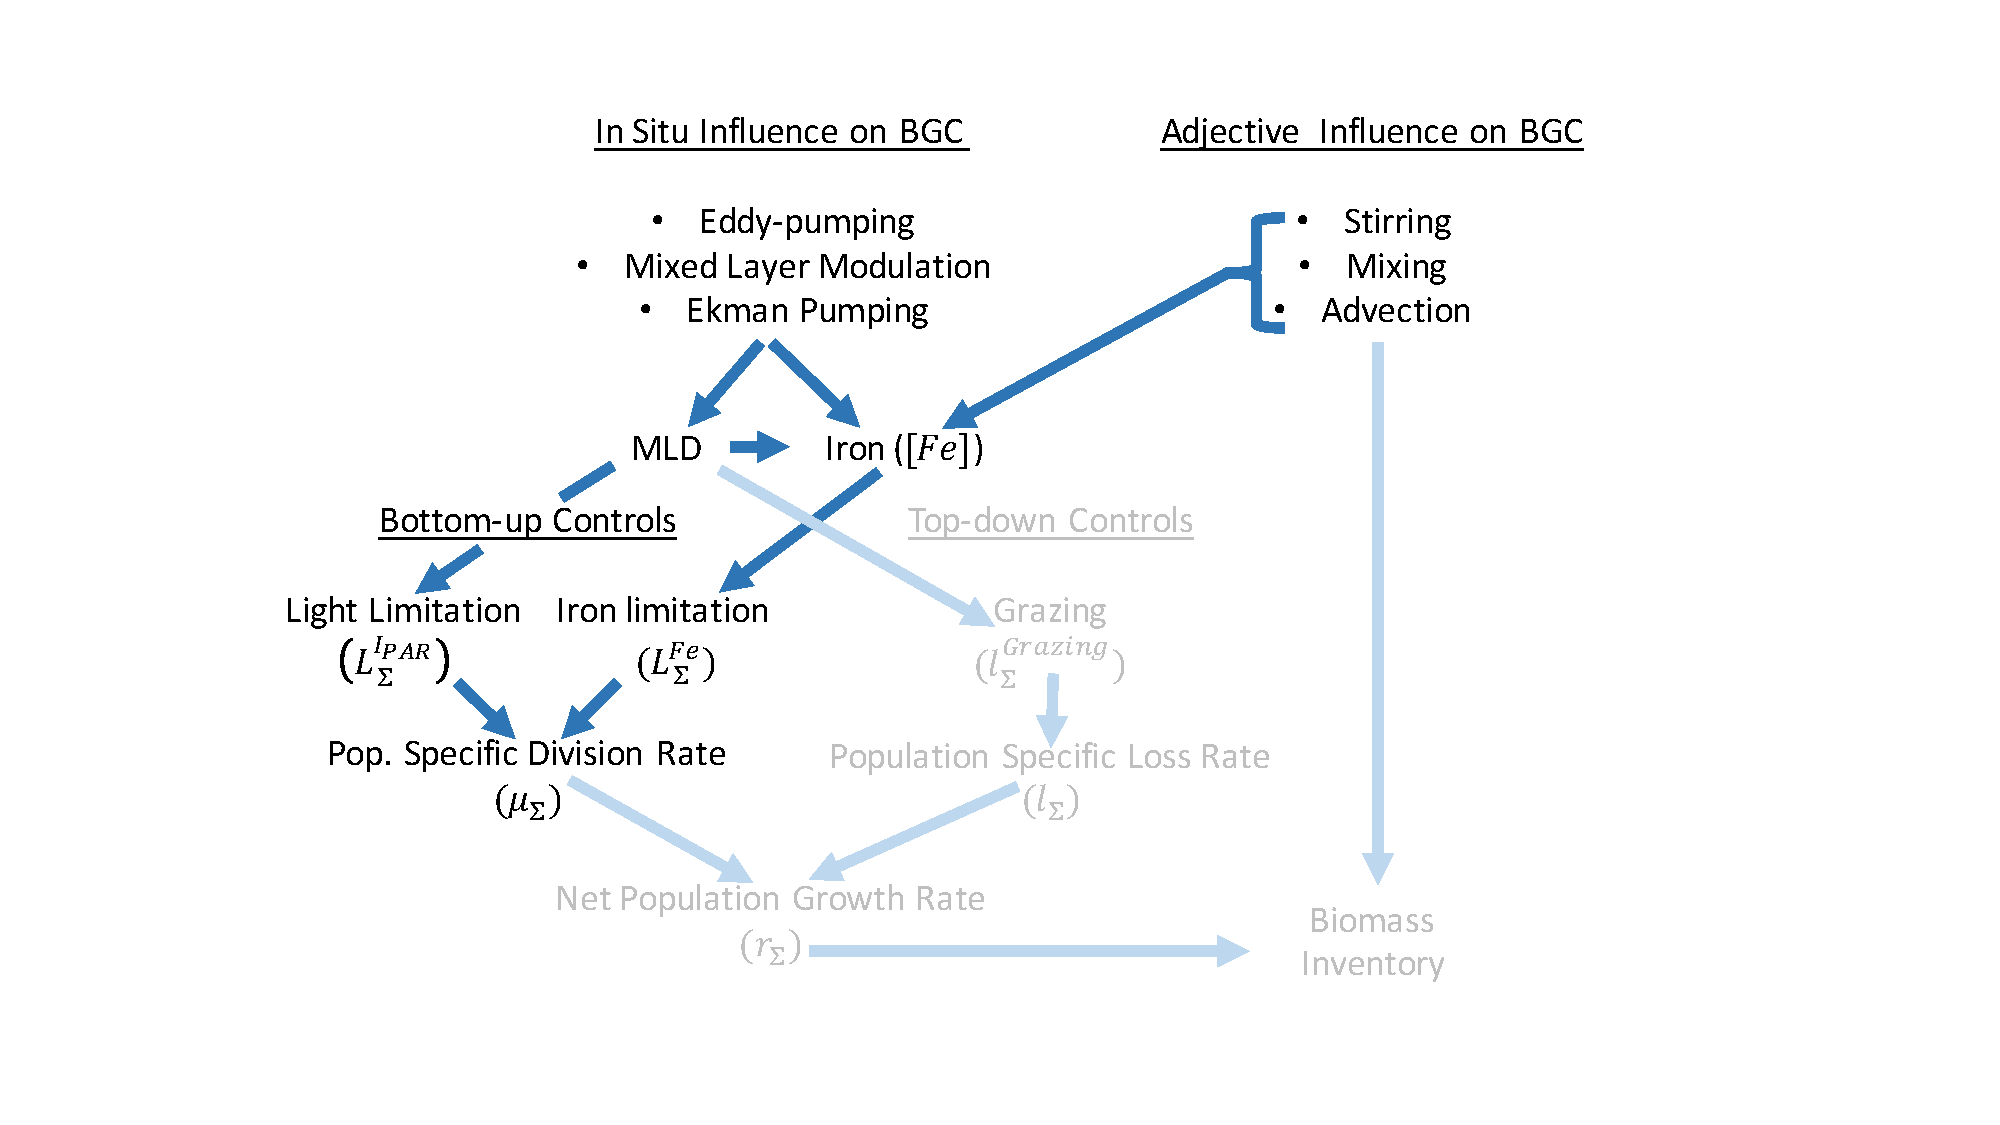
\includegraphics[scale=.8]{Fig1.pdf}
\end{adjustwidth}
\caption[Pathways for eddy influence on Biomass]
{\textbf{Figure 1.} Pathways for eddy influence on Biomass. (\textbf{MAY NOT INCLUDE}: but useful for organizing my thoughts.) Idealized flow chart of how physically induced processes in eddies can influence biogeochemistry, and ultimately biomass. Highlighted pathways and tracers are examined in this paper/Chapter 2. The others are examined in \textit{Rohr et. al} [in prep.]/Chapter 3 }
\label{fig:Fig1}
\end{figure}

%%%%%%%%%%%%%%%%%%%%%%%%
%%%%%% Figure 2 %%%%%%%%
%%%%%%%%%%%%%%%%%%%%%%%%

\begin{figure}[!htbp]
\begin{adjustwidth}{-1.2in}{-1.2in}
 \centering
 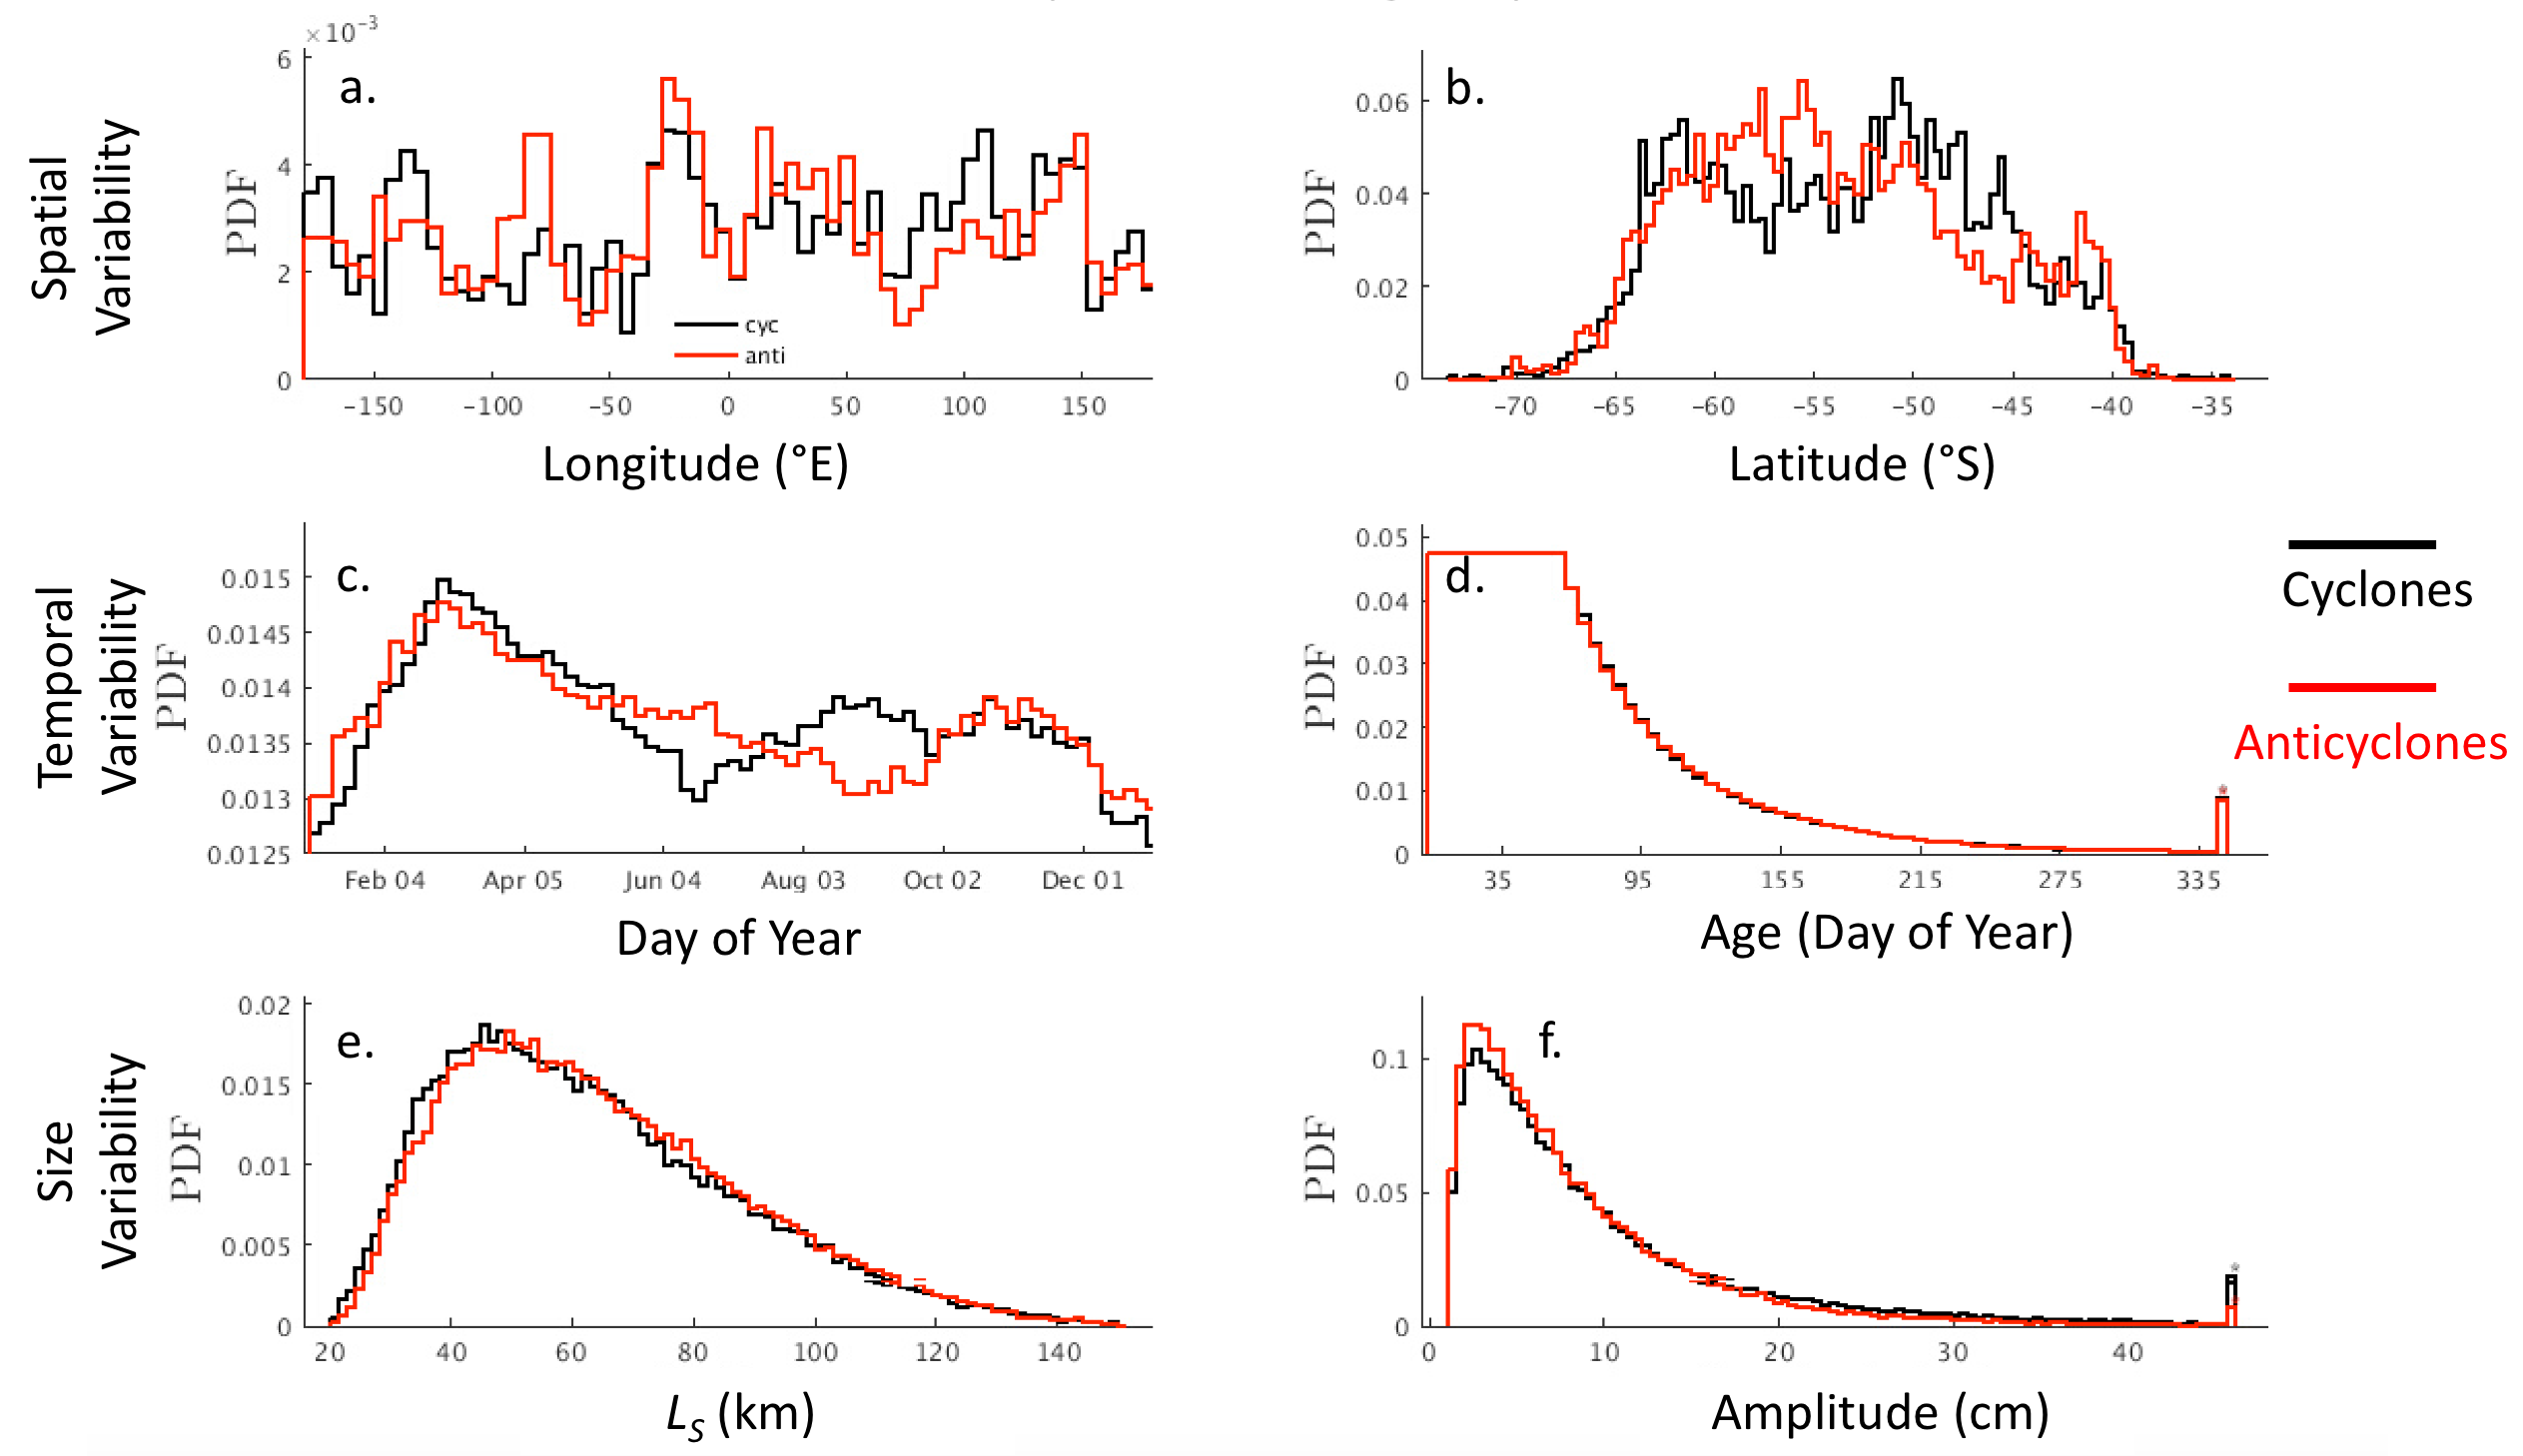
\includegraphics[scale=.40]{Fig2.png}
\end{adjustwidth}
\caption[Comparison of modeled and observed tracks and demographics]
{\textbf{Figure 2.} Place holder for Pete's track validation analysis. This figure will not be used, but it will be a similiar comparison on demographic distributions between obs and model}
\label{fig:Fig2}
\end{figure}


%%%%%%%%%%%%%%%%%%%%%%%%
%%%%%% Figure 3 %%%%%%%%
%%%%%%%%%%%%%%%%%%%%%%%%

\begin{figure}[!htbp]
 \begin{adjustwidth}{-2in}{-1.2in}
 \centering
 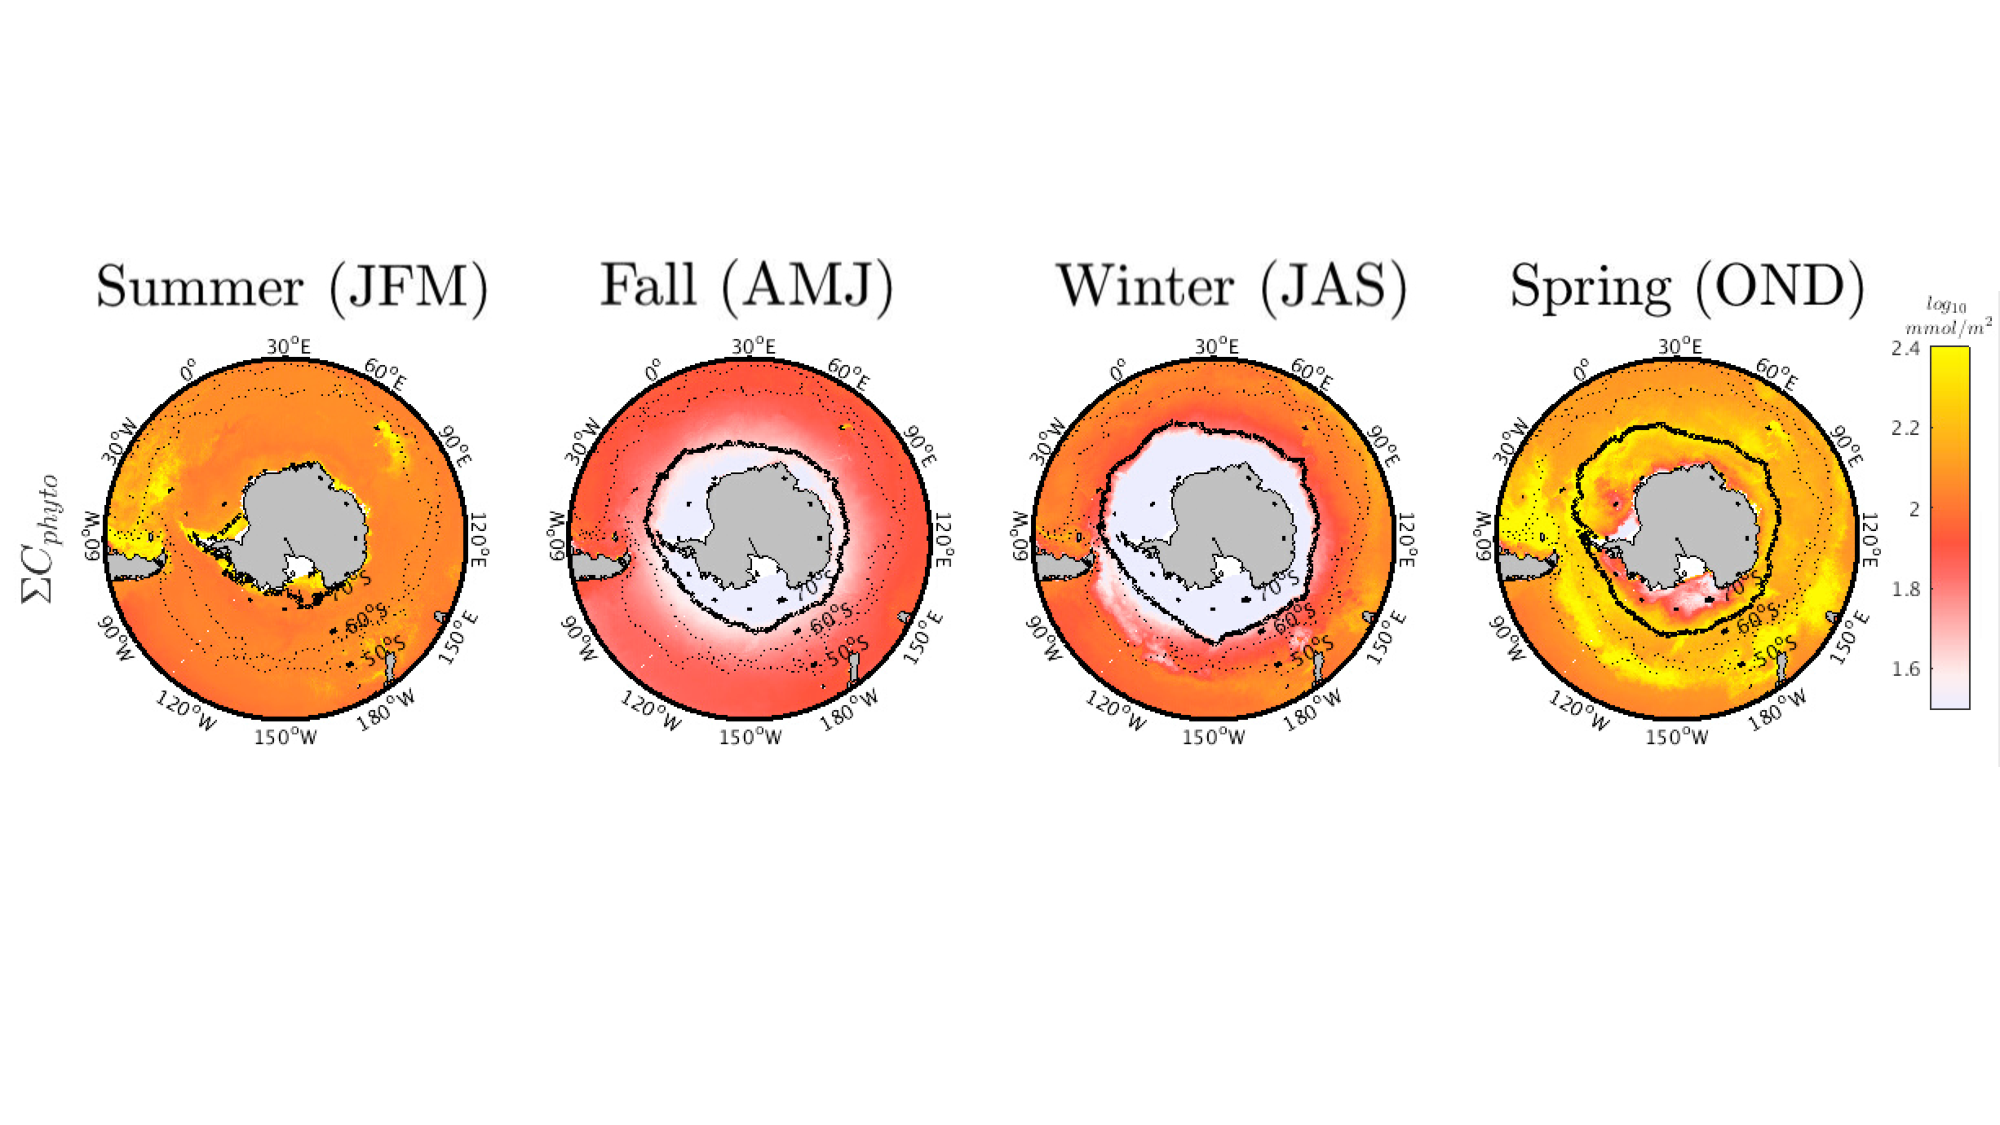
\includegraphics[scale=.80]{Fig3.pdf}
 \end{adjustwidth}
\caption[Seasonal climatology and eddy tracks. ]
{\textbf{Figure 3.} Seasonal Climatology and Eddy Tracks. (\textbf{a, b}) The simulated mean seasonal mixed layer depth ($\overline{MLD}$) and (\textbf{b, e}) deep iron differential ($\overline{\Delta[dFe]}$)) are plotted alongside (\textbf{c, f}) all coincident eddy tracks during the relevant seasonal window. Cyclonic (anticyclonic) eddy tracks are plotted in black (red). The mean 10\% ice contour is plotted in each subplot. (\textbf{a, b, c}) The shallow mixing "Summer" season comprising January-March (JFM) is plotted above and (\textbf{d, e, f}) the deep mixing 'Winter' season spanning July-September (JAS) is plotted below}
\label{fig:Fig3}
\end{figure}


%%%%%%%%%%%%%%%%%%%%%%%%
%%%%%% Figure 4 %%%%%%%%
%%%%%%%%%%%%%%%%%%%%%%%%

\begin{figure}[!htbp]
 \centering
 \begin{adjustwidth}{-1.5in}{-1.2in}
  \begin{tabular}{c c}
        \includegraphics[scale=.35]{Fig4a.pdf} &
        \includegraphics[scale=.35]{Fig4b.pdf} \\
        \includegraphics[scale=.35]{Fig4c.pdf} &
        \includegraphics[scale=.35]{Fig4d.pdf} \\
        \includegraphics[scale=.35]{Fig4e.pdf} & \\
  \end{tabular}
 \end{adjustwidth}
\caption[Seasonal and longitudinal distribution of eddy anomalies]
{\textbf{Figure 4.} Seasonal and longitudinal distribution of eddy anomalies. Mean eddy anomalies (averaged across the eddy surface area) for several tracers are plotted as a function of the climatologic day of occurrence (radial axis) and the longitude at which they formed (angular axis). Each time step from each track is included. "Overlapping" occurrences are averaged. Plots are smoothed with 2D loess filter a half power cutoff of 1 month in time (radial axis) and 6\degree in longitude (angular axis). Grid cells at which no eddy occurred over the 5 year run remain blank. Cyclones (anitcyclones) are included on the left (right) side of each subplot. Plots are included for (\textbf{a}) $MLD'$, (\textbf{b}) $[dFe]_\Sigma'$, (\textbf{c}) $(L_\Sigma^{I_{PAR}})'$,   (\textbf{d}) $(L_\Sigma^{Fe})'$, and (\textbf{e}) $\mu_\Sigma'$}
\label{fig:Fig4}
\end{figure}

%%%%%%%%%%%%%%%%%%%%%%%%
%%%%%% Figure 5 %%%%%%%%
%%%%%%%%%%%%%%%%%%%%%%%%

\begin{figure}[!htbp]
    \begin{adjustwidth}{-2.2in}{-1.2in}
    \centering
        \includegraphics[scale=.8]{Fig6.pdf}
    \end{adjustwidth}
    \caption[{Distribution of $[dFe]_\Sigma'$.}]
    {\textbf{Figure 5.} Distribution of $[dFe]_\Sigma'$. The mean magnitude (with +/-1 standard deviation shaded) of $MLD'$ for cyclones (black) and anticyclones (red) is plotted as a function of (\textbf{a}) Longitude ($\degree E$), (\textbf{b}) Latitude ($\degree S$), (\textbf{c}) Day of Year, (\textbf{d}) Eddy Age ($days$), (\textbf{e}) Eddy Radius ($km$), (\textbf{f}) Eddy Amplitude ($cm$), (\textbf{g}) $MLD_{Clim}$ ($m$), (\textbf{h}) $Ice_{Clim}$ ($\%$), (\textbf{i}) $\Delta[dFe]_{Clim}$ ($\%$),and (\textbf{j}) $MLD'$. Outlier eddies in the top/bottom .5 percentile of $[dFe]_\Sigma'$ were removed.}
\label{fig:Fig5}
\end{figure}



%%%%%%%%%%%%%%%%%%%%%%%%
%%%%%% Figure 6 %%%%%%%%
%%%%%%%%%%%%%%%%%%%%%%%%

\begin{figure}[!htbp]
    \begin{adjustwidth}{-2.2in}{-1.2in}
    \centering
        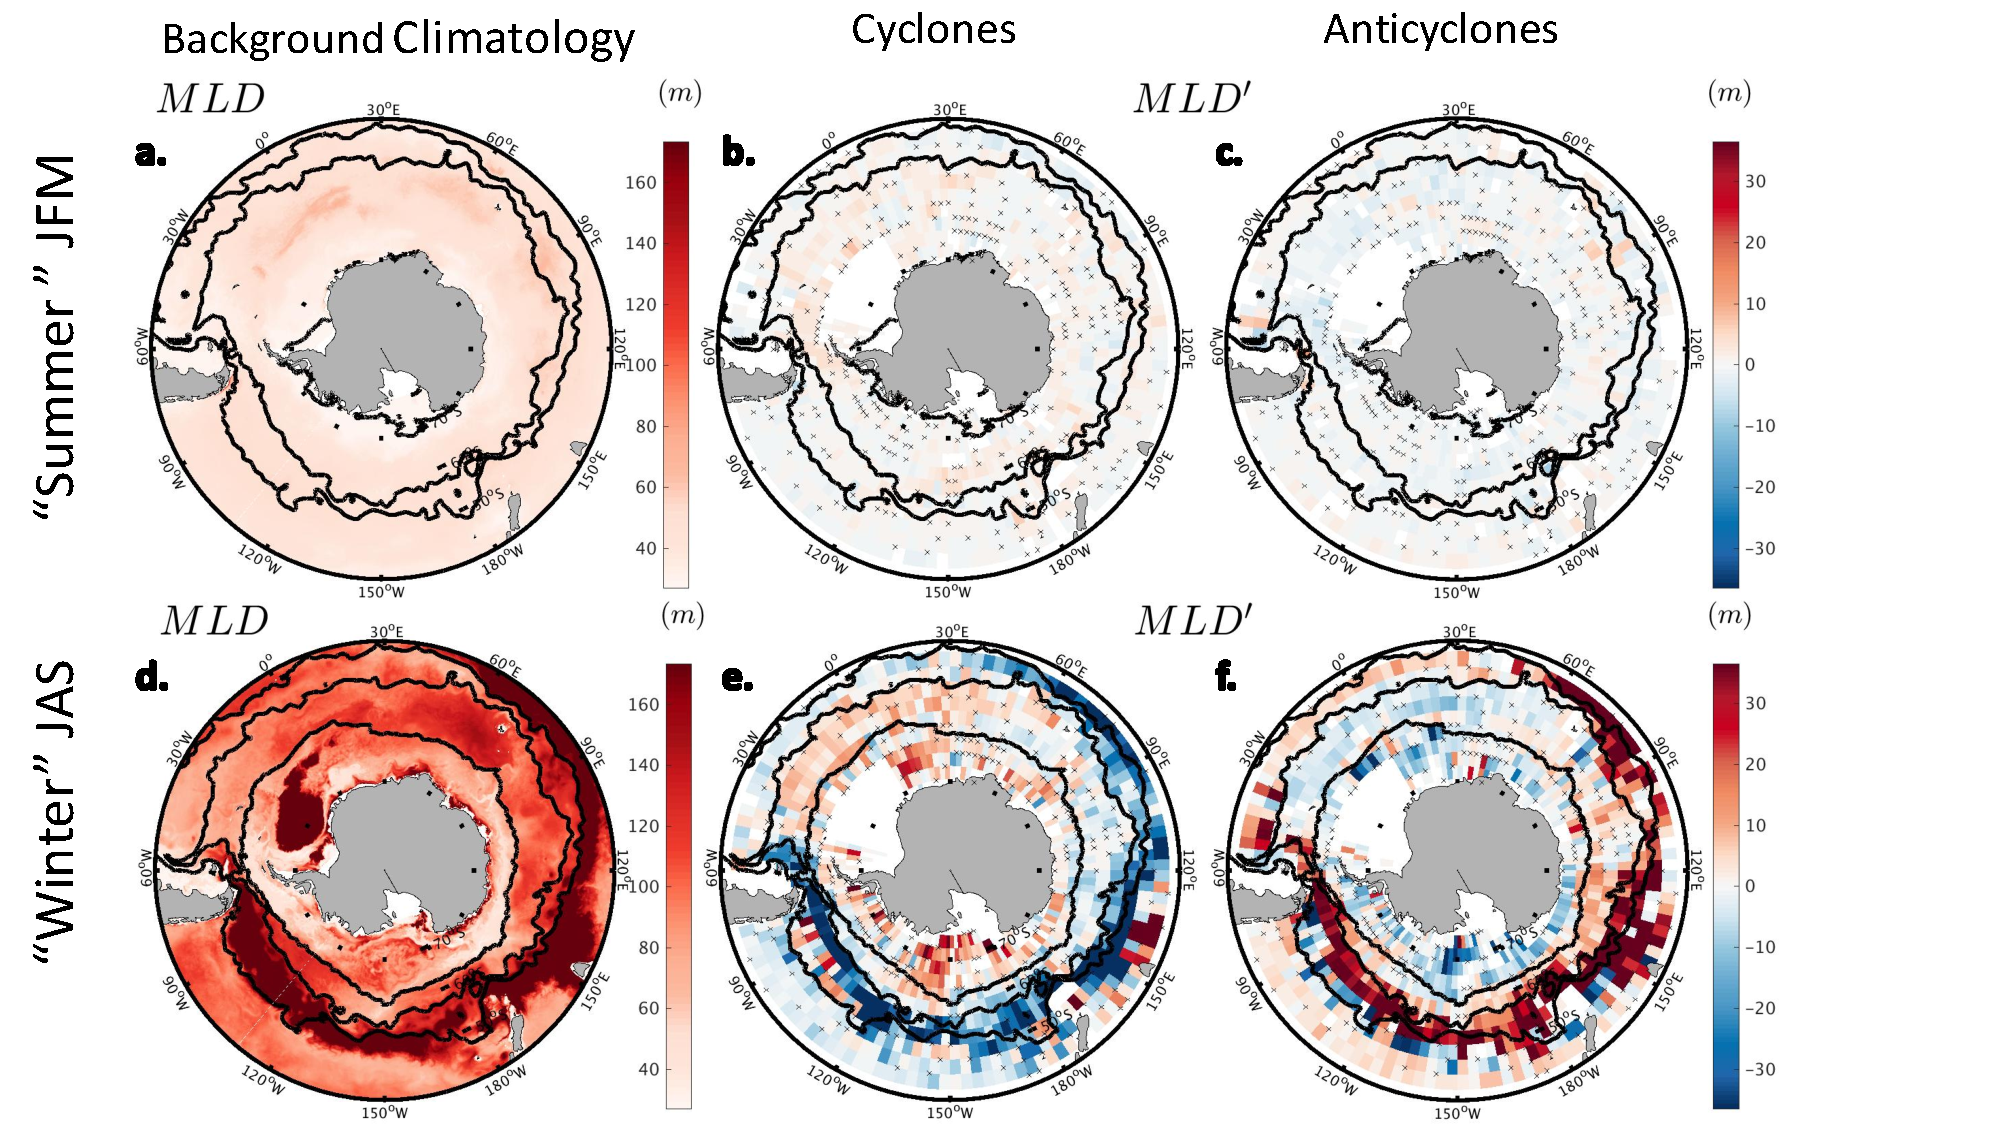
\includegraphics[scale=.8]{Fig5.pdf}
    \end{adjustwidth}
    \caption[Distribution of $MLD'$.]
    {\textbf{Figure 6.} Distribution of $MLD'$. The mean magnitude (with +/-1 standard deviation shaded) of $MLD'$ for cyclones (black) and anticyclones (red) is plotted as a function of (\textbf{a}) Longitude ($\degree E$), (\textbf{b}) Latitude ($\degree S$), (\textbf{c}) Day of Year, (\textbf{d}) Eddy Age ($days$), (\textbf{e}) Eddy Radius ($km$), (\textbf{f}) Eddy Amplitude ($cm$), and (\textbf{g}) $MLD_{Clim}$ ($m$), (\textbf{h}) $Ice_{Clim}$ ($\%$). Outlier eddies in the top/bottom .5 percentile of $MLD'$ were removed.}
\label{fig:Fig6}
\end{figure}




%%%%%%%%%%%%%%%%%%%%%%%%
%%%%%% Figure 7 %%%%%%%%
%%%%%%%%%%%%%%%%%%%%%%%%

\begin{figure}[!htbp]
    \begin{adjustwidth}{-3.6in}{-1.2in}
    \centering
        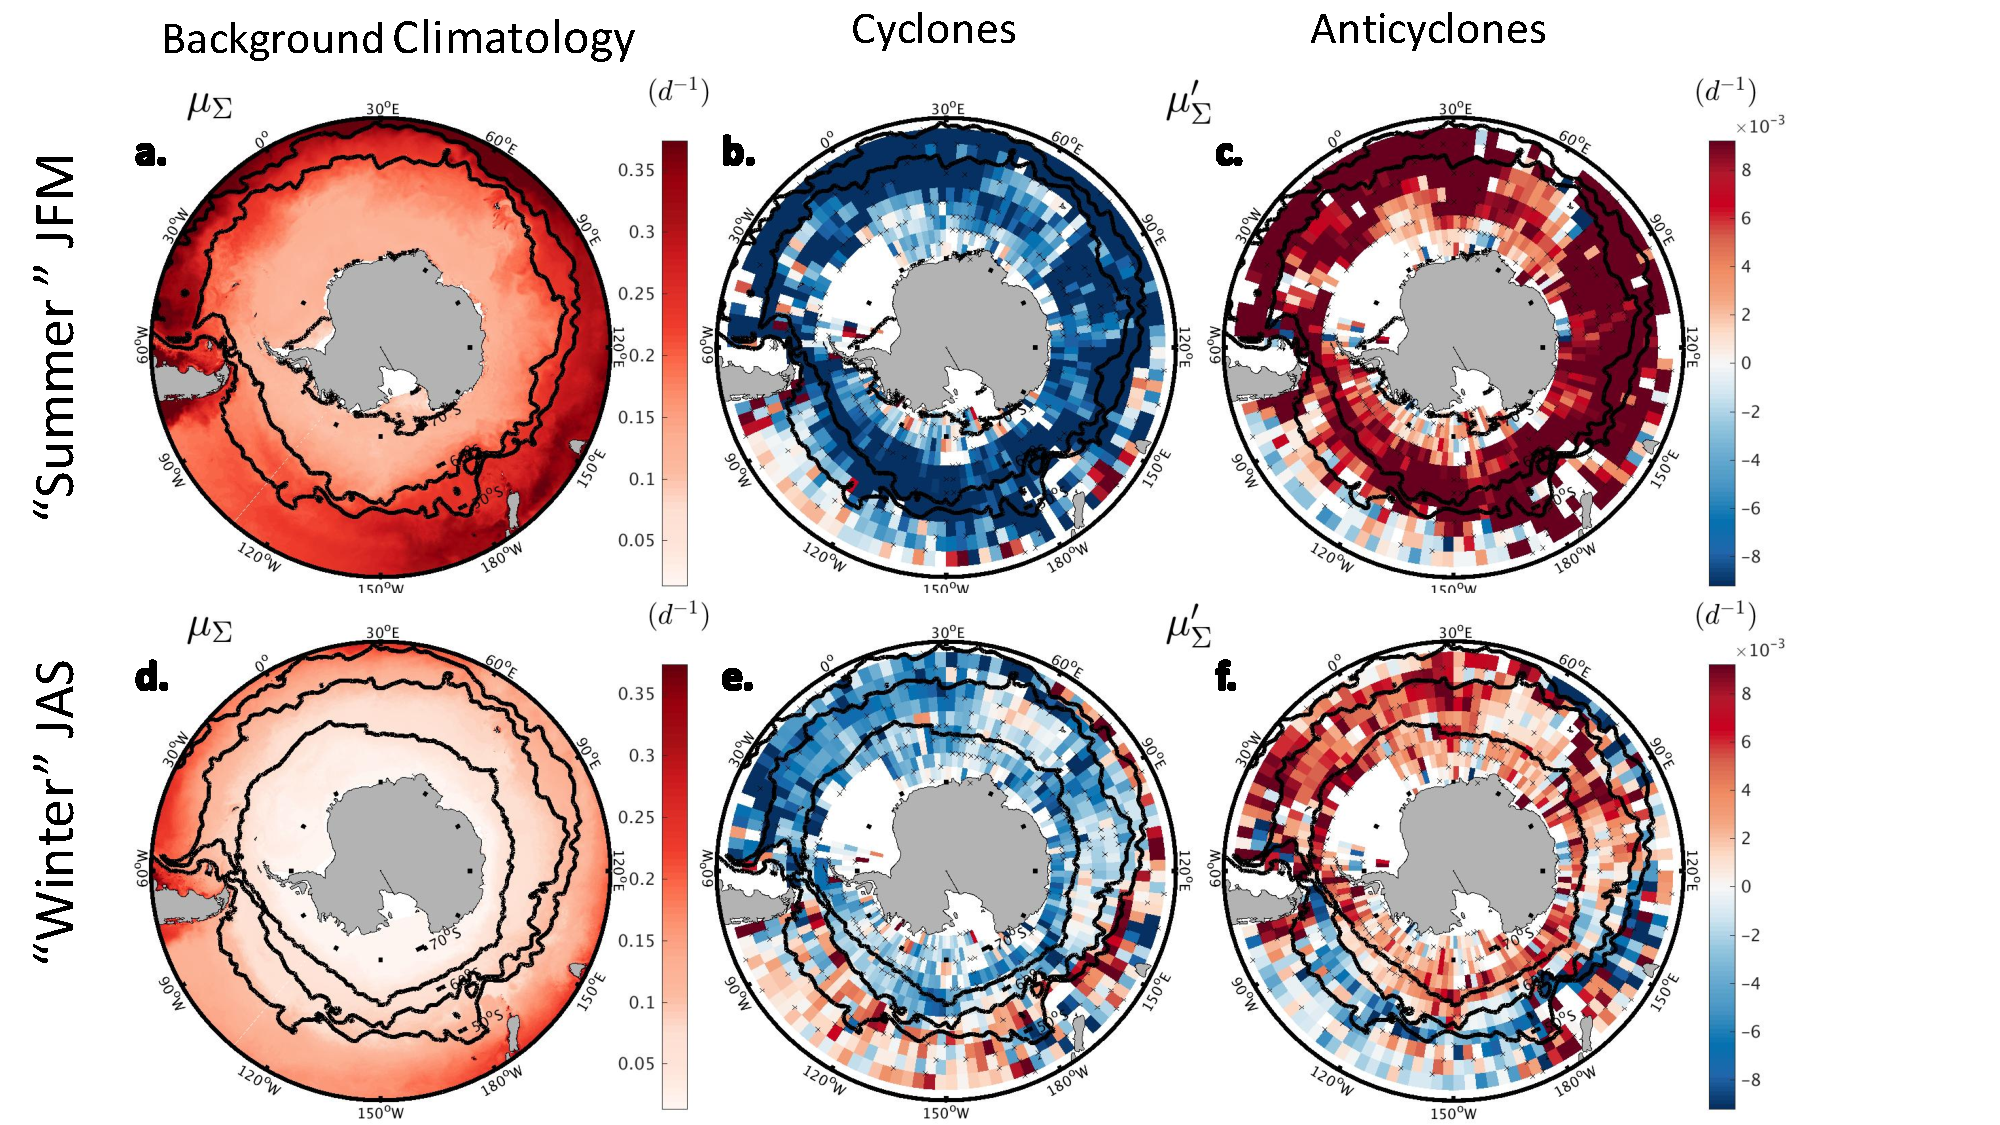
\includegraphics[scale=1]{Fig7.pdf}
    \end{adjustwidth}
    \caption[Variability in vertical mixing iron transport anomalies]
    {\textbf{Figure 7.} Variability in vertical mixing iron transport anomalies. The depth profile of anomalous iron transport via vertical diabatic mixing $Mix'_{Fe}$ is plotted as a of (\textbf{a, b}) Longitude ($\degree E$), (\textbf{c, d}) Latitude ($\degree S$), the (\textbf{e, f}) $MLD_{Clim}$ ($m$), (\textbf{g, h}) $Ice_{Clim}$ ($\%$), (\textbf{i, j}) $\Delta[dFe]_{Clim}$ ($\%$),and (\textbf{k, l}) $MLD'$.Cyclones are plotted on the left (\textbf{a, c, e, g, i, k}) and anticyclones are plotted on the right (\textbf{b, d, f, h, j, l}). Outlier eddies in the top/bottom .5 percentile of $[dFe]_\Sigma'$ were removed. }
\label{fig:Fig7}
\end{figure}




%%%%%%%%%%%%%%%%%%%%%%%%
%%%%%% Figure 8 %%%%%%%%
%%%%%%%%%%%%%%%%%%%%%%%%

\begin{figure}[!htbp]
    \begin{adjustwidth}{-3.6in}{-1.2in}
    \centering
        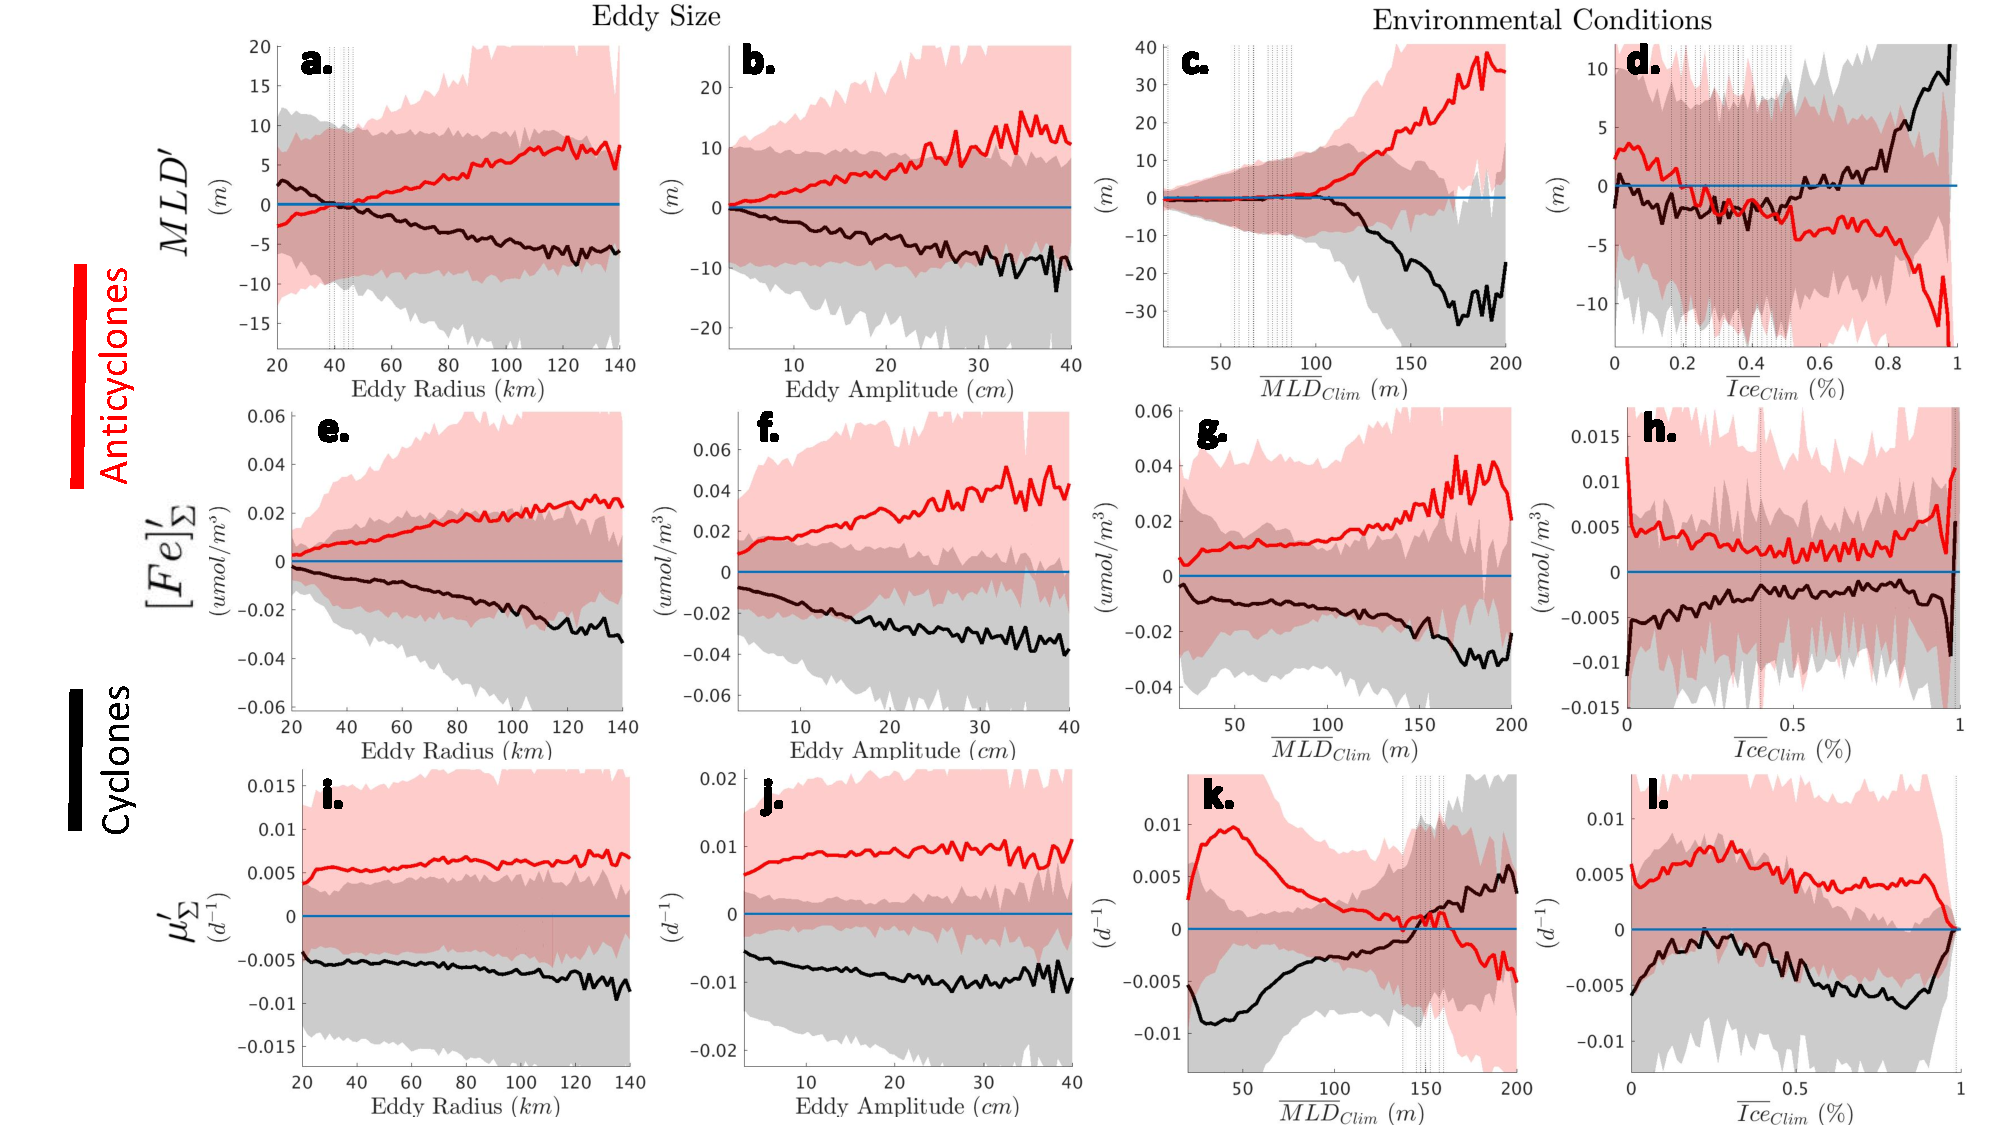
\includegraphics[scale=1]{Fig8.pdf}
    \end{adjustwidth}
    \caption[Variability in vertical advection iron transport anomalies]
    {\textbf{Figure 8.} Variability in vertical advection iron transport anomalies. The depth profile of anomalous iron transport via vertical advection ($W'_{Fe}$) is plotted as a function of (\textbf{a, b}) Longitude ($\degree E$), (\textbf{c, d}) Latitude ($\degree S$), the (\textbf{e, f}) $MLD_{Clim}$ ($m$), (\textbf{g, h}) $Ice_{Clim}$ ($\%$), (\textbf{i, j}) $\Delta[dFe]_{Clim}$ ($\%$),and (\textbf{k, l}) $MLD'$.Cyclones are plotted on the left (\textbf{a, c, e, g, i, k}) and anticyclones are plotted on the right (\textbf{b, d, f, h, j, l}). Outlier eddies in the top/bottom .5 percentile of $[dFe]_\Sigma'$ were removed. }
\label{fig:Fig8}
\end{figure}


%%%%%%%%%%%%%%%%%%%%%%%%
%%%%%% Figure 9s %%%%%%%%
%%%%%%%%%%%%%%%%%%%%%%%%

\begin{figure}[!htbp]
 \centering
 \begin{adjustwidth}{-1in}{0in}
  \begin{tabular}{c }
        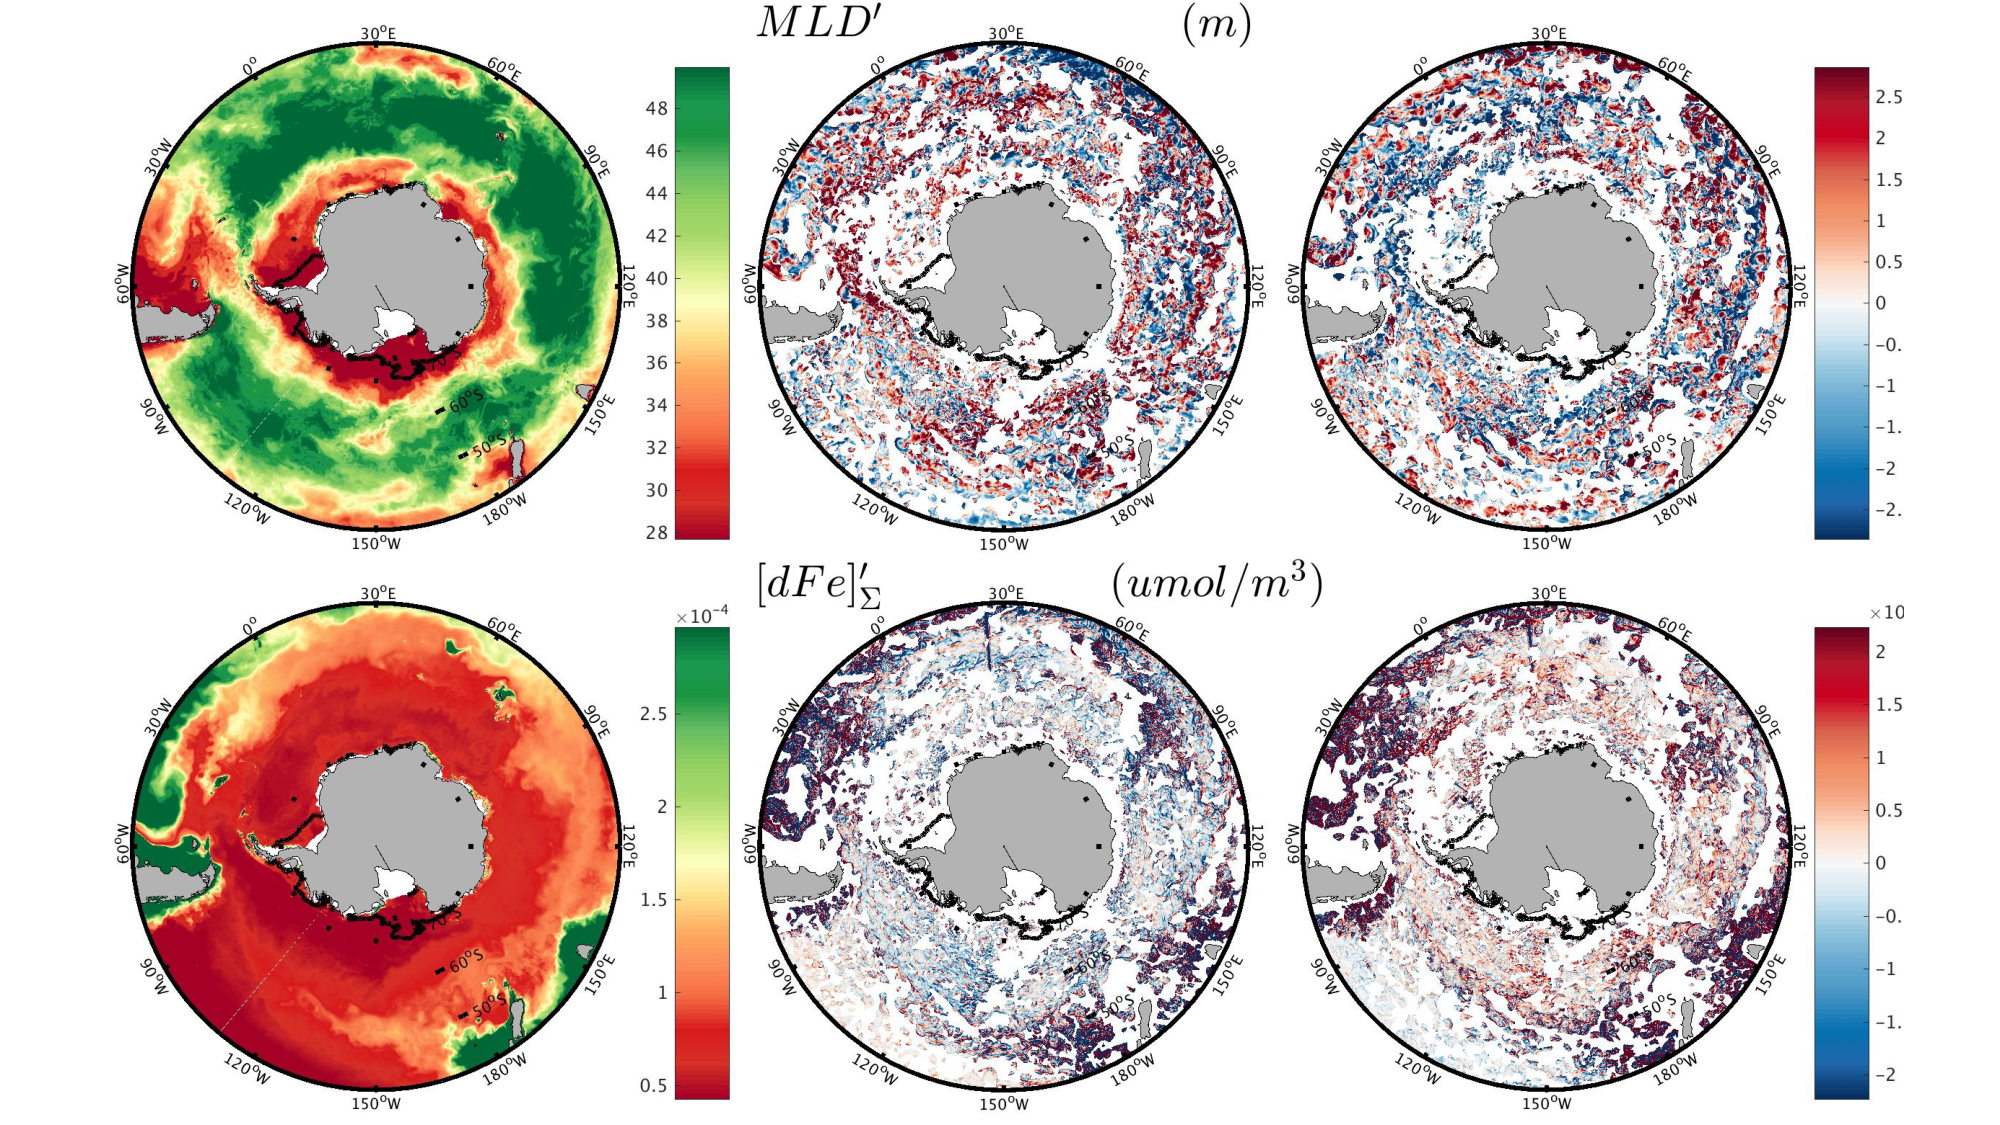
\includegraphics[scale=.6]{Fig9/Not_Smoothed/Fig9a_s.pdf} \\
        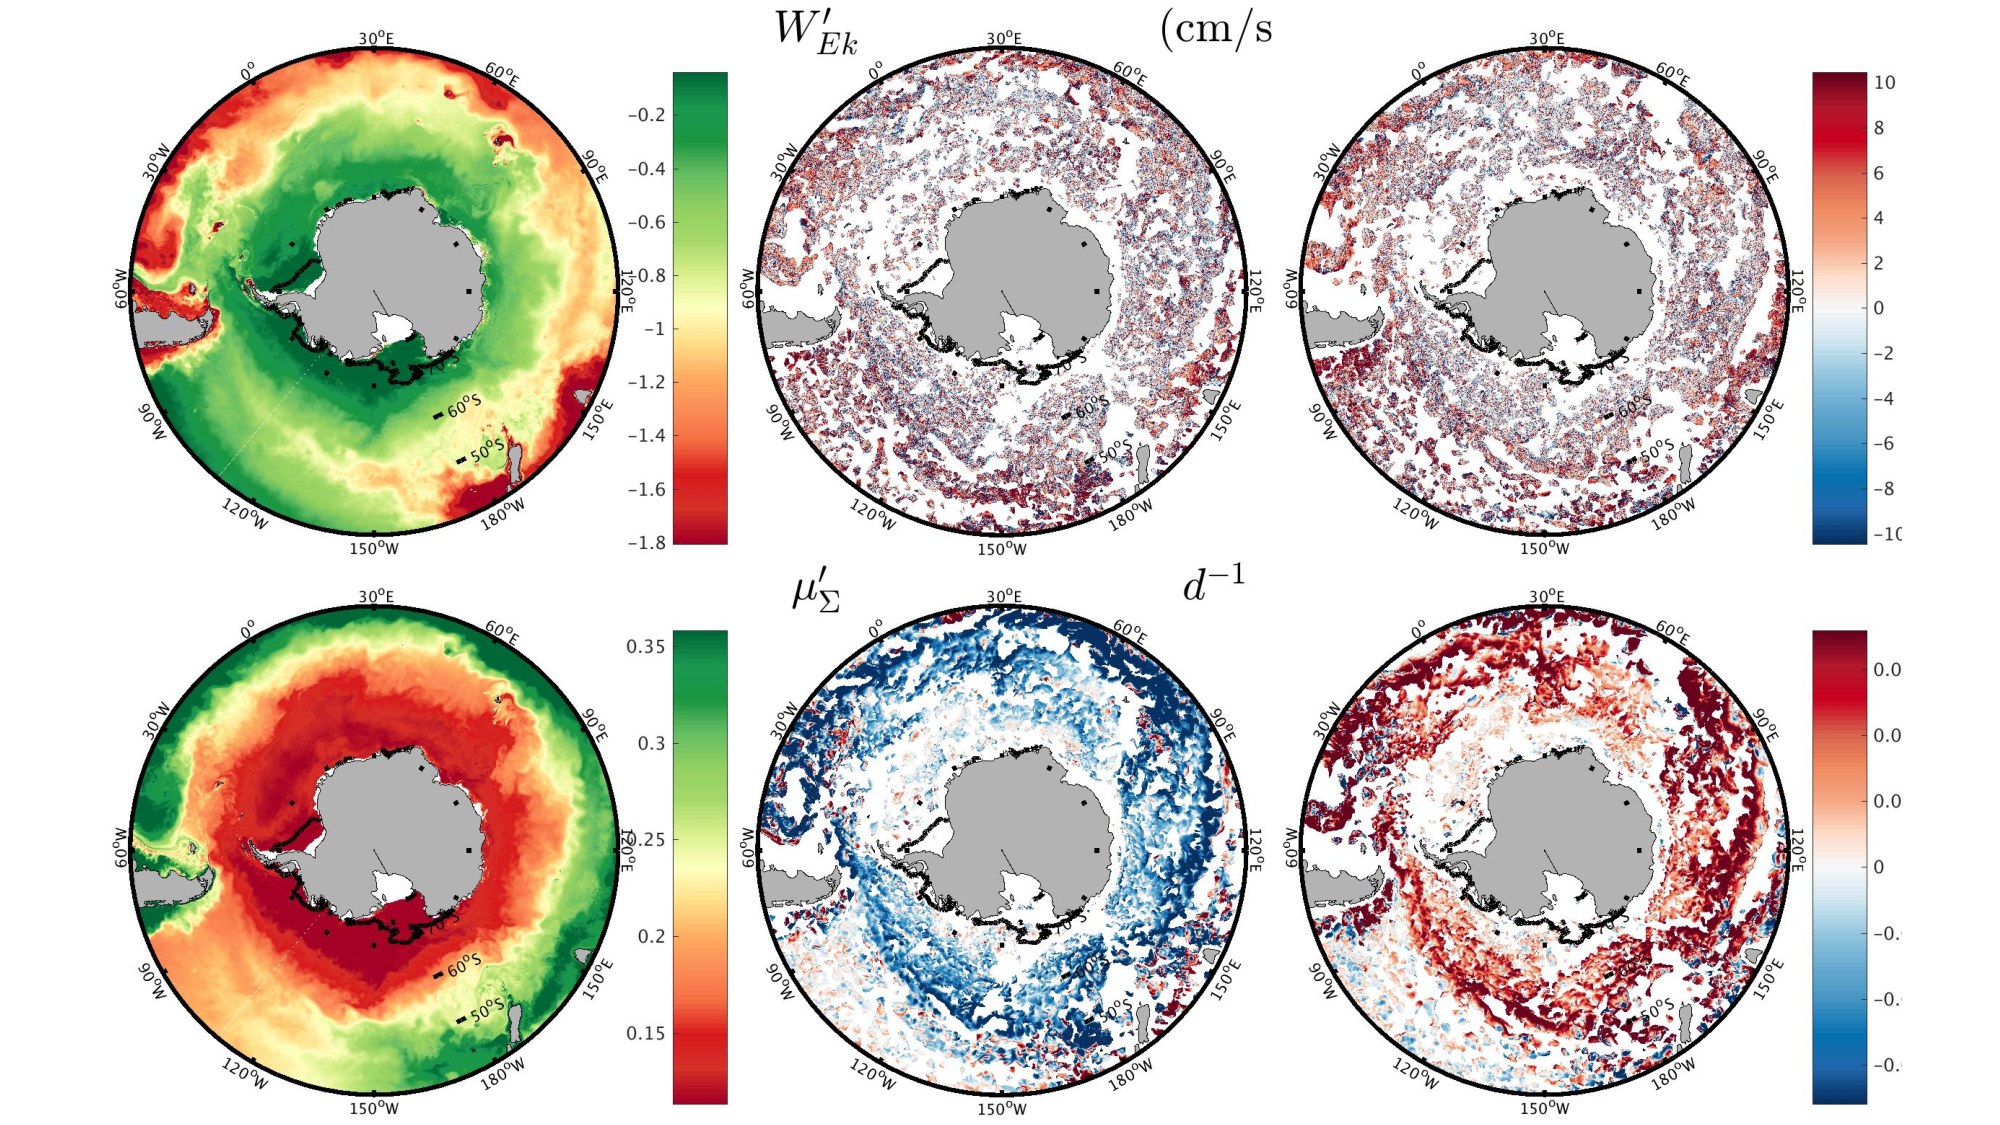
\includegraphics[scale=.6]{Fig9/Not_Smoothed/Fig9b_s.pdf} \\
    
  \end{tabular}
 \end{adjustwidth}
\caption[Figure Title]
{\textbf{Figure 9.} Figure Title
}
\label{fig:Fig9}
\end{figure}

%%%%%%%%%%%%%%%%%%%%%%%%
%%%%%% Figure 9w %%%%%%%%
%%%%%%%%%%%%%%%%%%%%%%%%

\begin{figure}[!htbp]
 \centering
 \begin{adjustwidth}{-1in}{0in}
  \begin{tabular}{c }
        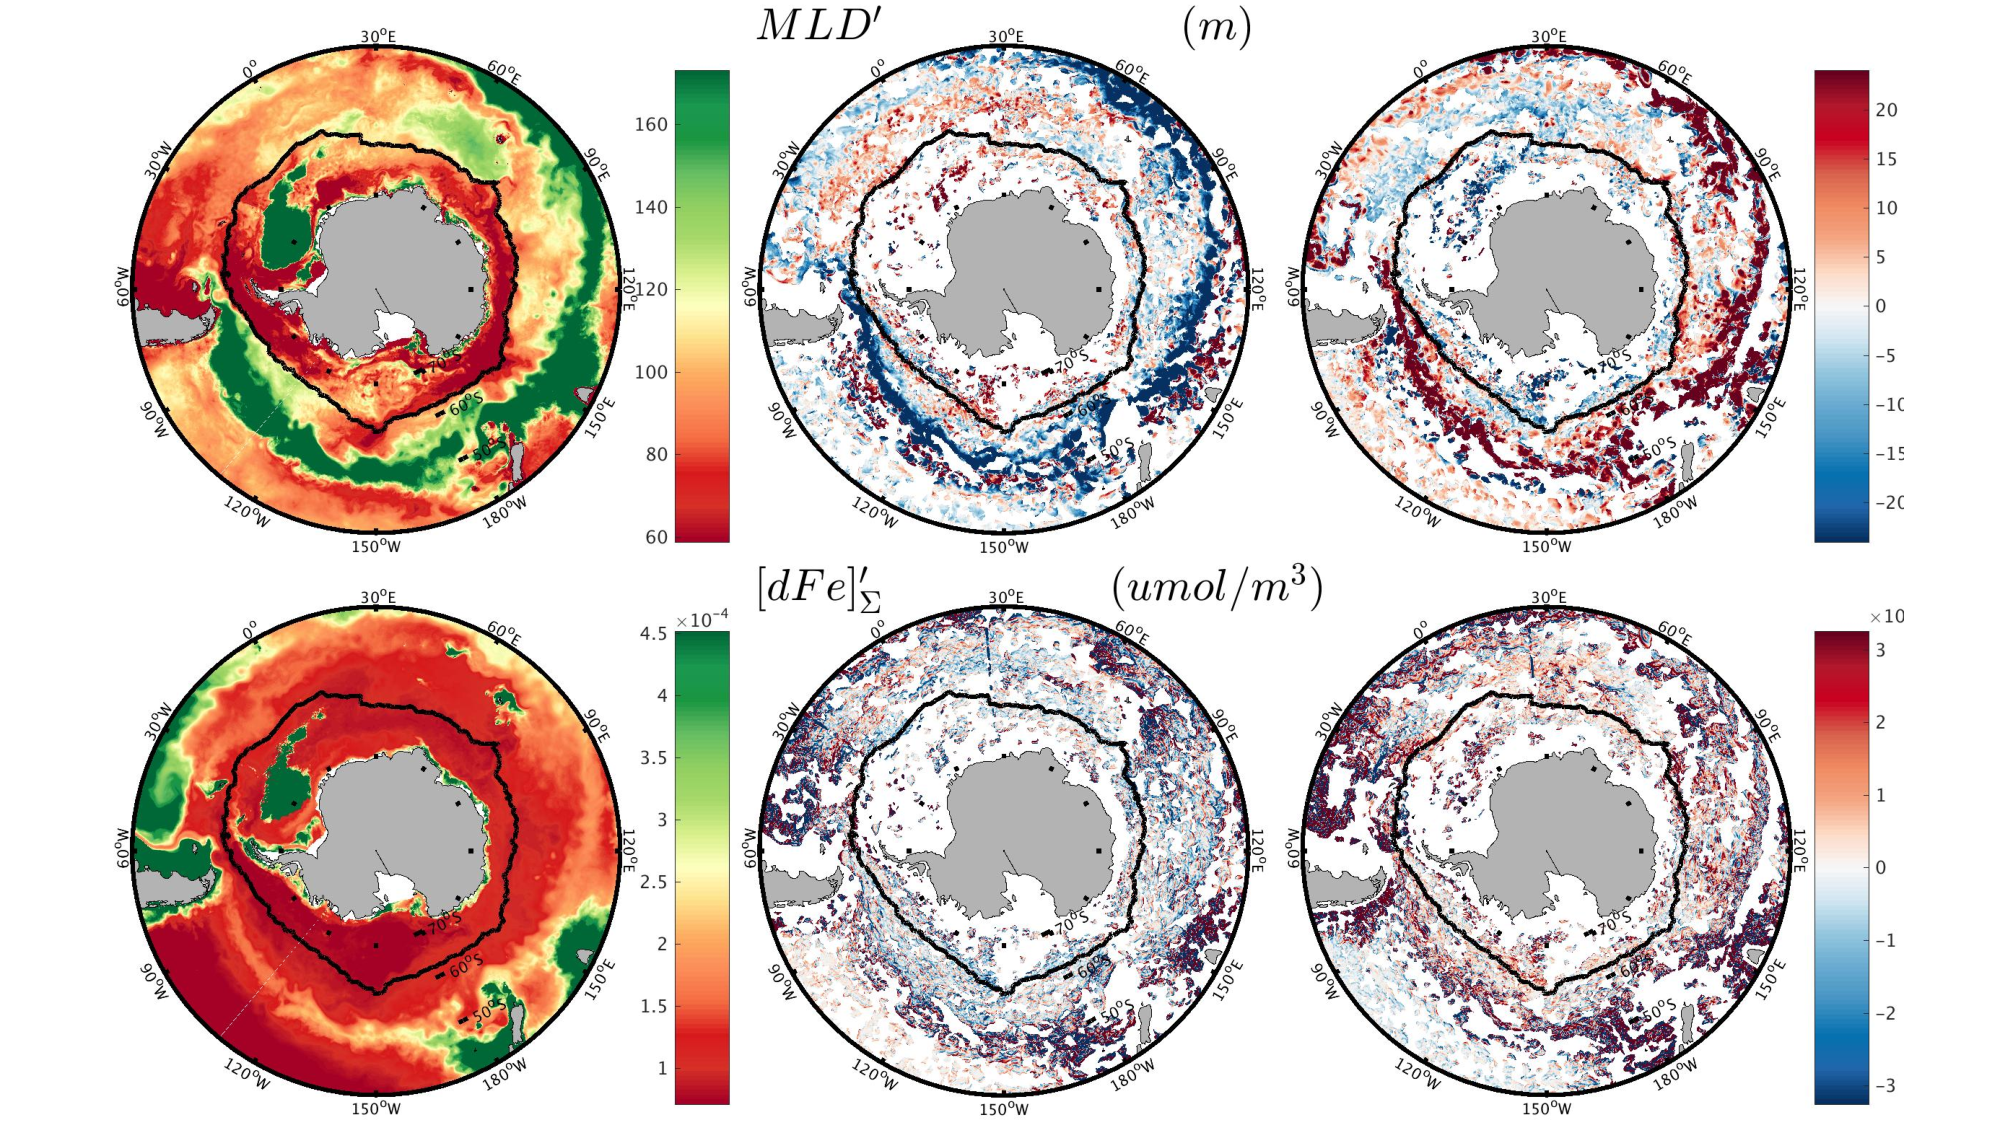
\includegraphics[scale=.6]{Fig9/Not_Smoothed/Fig9a_w.pdf} \\
        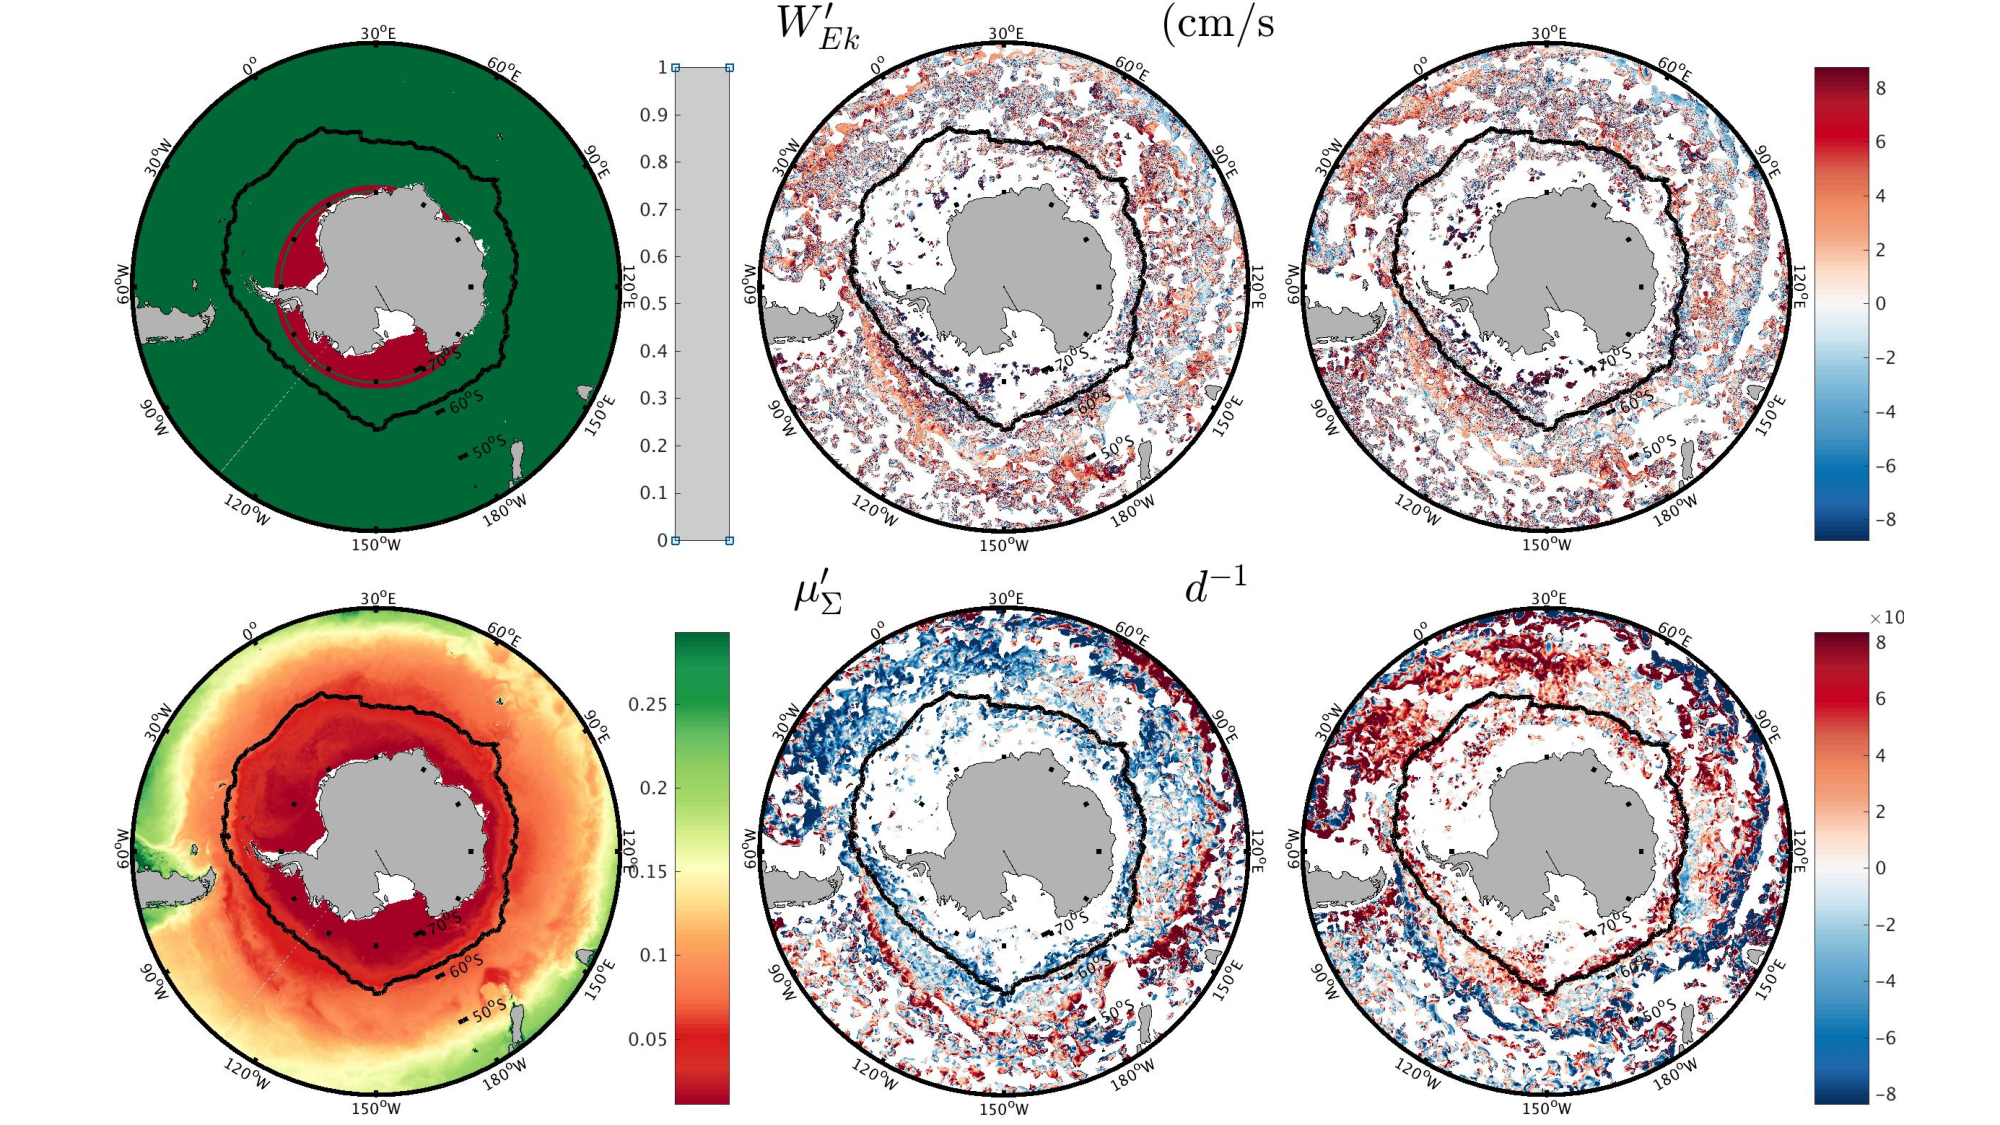
\includegraphics[scale=.6]{Fig9/Not_Smoothed/Fig9b_w.pdf} \\
    
  \end{tabular}
 \end{adjustwidth}
\caption[Figure Title]
{\textbf{Figure 9.} Figure Title
}
\label{fig:Fig9}
\end{figure}


%%%%%%%%%%%%%%%%%%%%%%%
%% Potential Figures %%
%%%%%%%%%%%%%%%%%%%%%%%
\begin{comment}

%%%%%%%%%%%%%%%%%%%%%%%%
%%%%%% Figure 9 %%%%%%%%
%%%%%%%%%%%%%%%%%%%%%%%%

\begin{figure}[!htbp]
    \begin{adjustwidth}{-1.2in}{-1.2in}
    \centering
        \includegraphics[scale=.40]{holder.png}
    \end{adjustwidth}
    \caption[division rates]
    {\textbf{Figure 9.} division rate }
\label{fig:Fig9}
\end{figure}


%%%%%%%%%%%%%%%%%%%%%%%%
%%%%%% Figure 10 %%%%%%%%
%%%%%%%%%%%%%%%%%%%%%%%%

\begin{figure}[!htbp]
    \begin{adjustwidth}{-1.2in}{-1.2in}
    \centering
        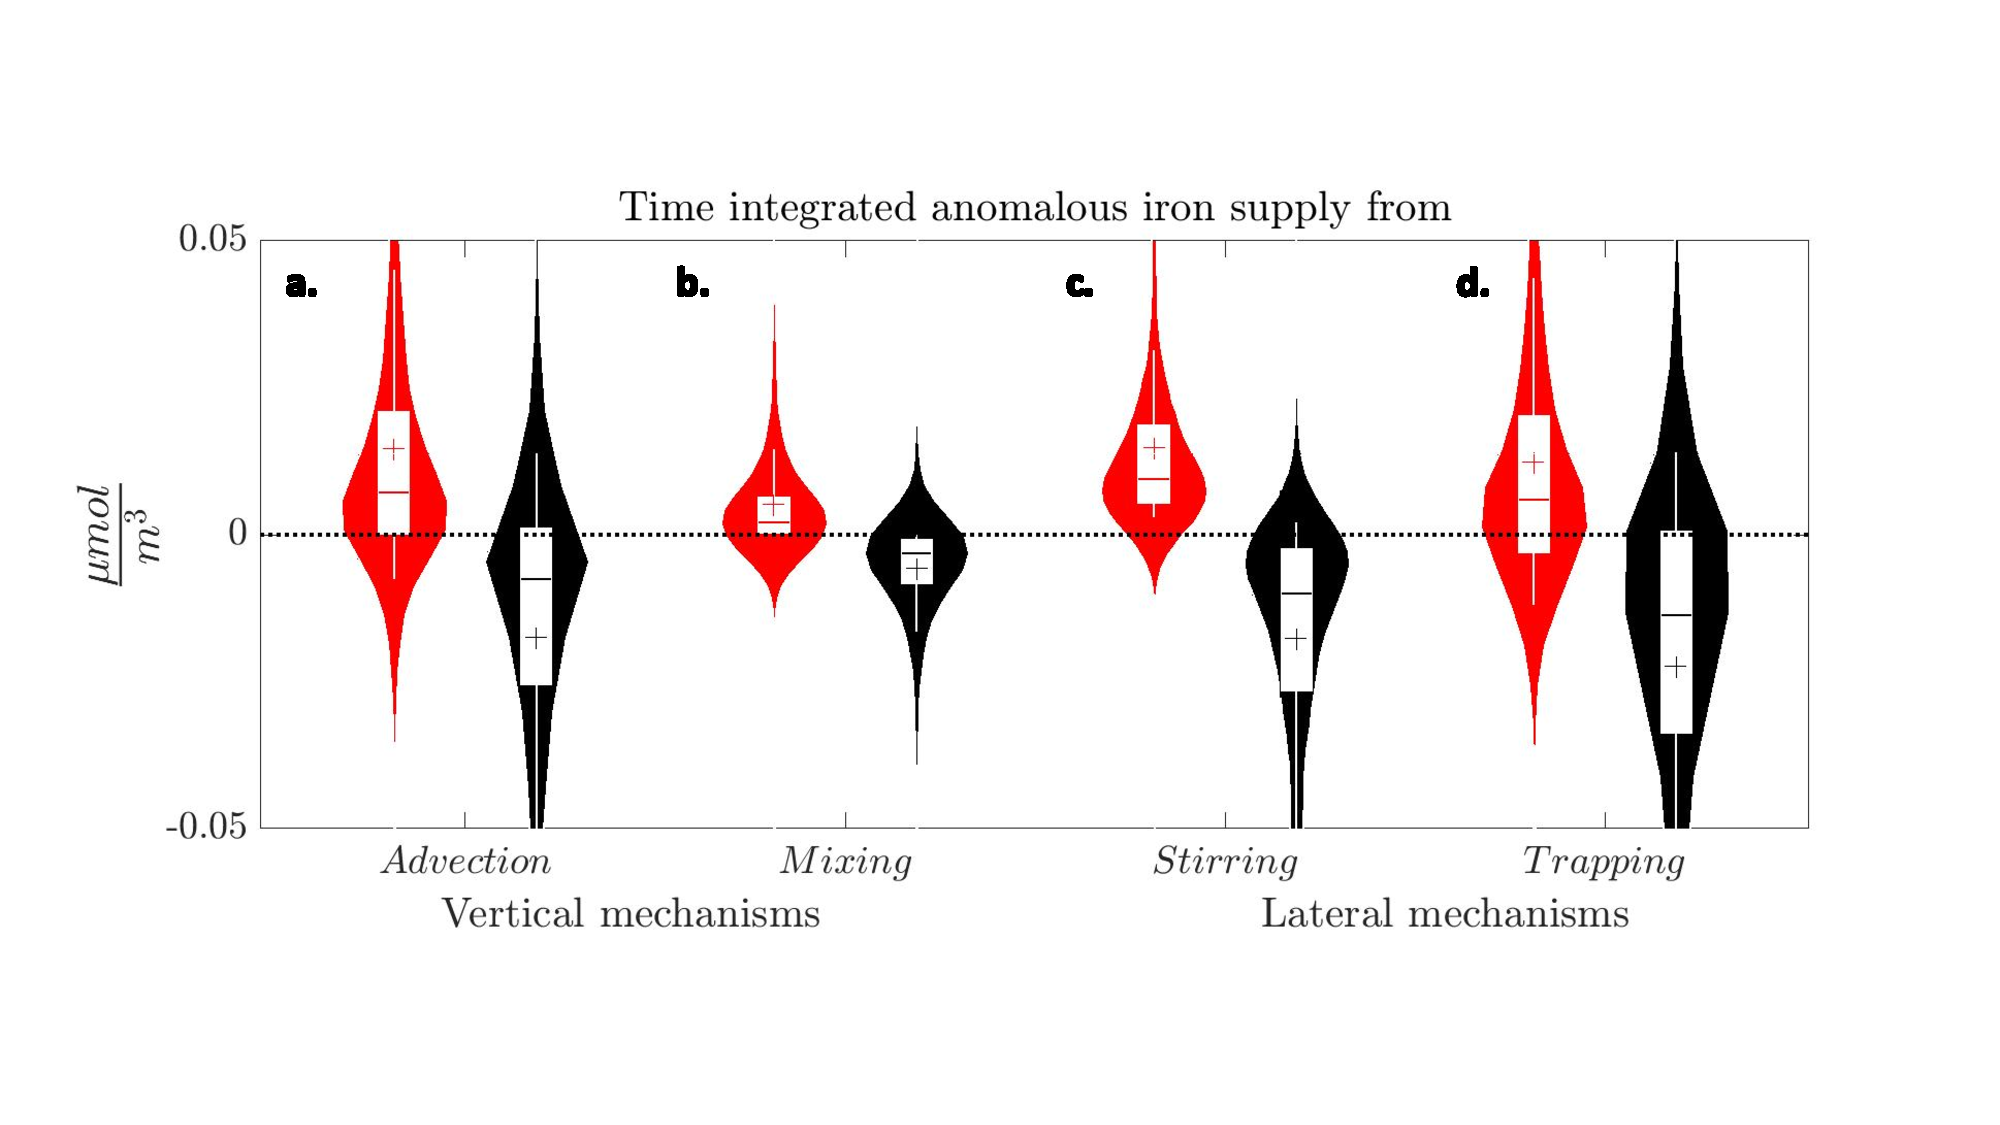
\includegraphics[scale=.40]{Fig9.png}
    \end{adjustwidth}
    \caption[Regional Composite of Eddies in Deep Mixing Pacific.]
    {\textbf{Figure 10.} Regional Composite of Eddies in Deep Mixing Pacific. The seasonal progression of $MLD'$, $[TotFe]_\Sigma'$,  $(L_\Sigma^{I_{PAR}})'$, $(L_\Sigma^{Fe})'$, and  $\mu_\Sigma'$, is plotted on the left for cyclones and right for anticyclones. Each figure gridcell represents the average of all model grid cell anomalies within eddies of the specified polarity during the specified month. Above, the climatologic background mixed layer depth and ice fraction for the bounded region are plotted. The region is defined as north of 58\degree S, south of 48\degree S, west of 95\degree W, and east of 180\degree W. Note that $MLD'$ and $[TotFe]_\Sigma'$ are scaled to fit on the colorbar.}
\label{fig:Fig10}
\end{figure}

\end{comment}










%%%%%%%%
% Notes For Scott
%%%%%%%%
\newpage

%Key Points
% Key Points
\vspace{5mm}
\subsubsection*{Key Points}
\vspace{5mm}
\begin{itemize}
\item  Phytoplankton division rates are generally deflated in cyclones and inflated in anticyclones 
\item The division rate anomaly is driven by increased (reduced) iron stress in cyclones (anticylones). Light limitation plays a less significant, often competing, role.
\item  $[dFe]_\Sigma'$ is predominately negative in cyclones and positive in anticyclones. This is opposite the direction that eddy pumping would induce, requiring a different dominant iron transport pathway: likely either $MLD$ modification or Ekman pumping
\item Roughly 50\% of all cyclones (anticyclones), notably larger eddies subject to deep background mixing (See Fig 6, Table 1), experience shallower (deeper) $MLD$ and detrain (entrain) iron (See Fig.7). This helps explain the simulated direction of $[dFe]_\Sigma'$.
\item There are, however, many eddies, particularly smaller ones with weaker background mixing, that exhibit a mixing anomaly in opposition to the direction of $[dFe]_\Sigma'$, suggesting a different, polarity dependent, iron flux. 
\item The vertical flux of iron via advection (Fig. 8), is roughly 2-4 times as strong as the vertical flux of iron via mixing (Fig. 7), suggesting a dominant, adjective pathway for iron transport in eddies, likely Ekman pumping. 
\end{itemize}
%

% NOTES
\subsubsection*{NOTES}
\vspace{5mm}
\begin{itemize}
    \item I have replaced $[TotFe]$ (the sum of all iron pools) with $[dFe]$ (just the dissolved iron) as it dominates the iron budget, doesnt change the results, and is simpler.
    \item I have introduced a new metric - deep iron differential ($\Delta[dFe]$) - to quantify the concentration of iron below the mixed layer relative to the mixed layer concentration. The goal is to understand what an eddy-modifed mixed layer is tapping into. $\Delta[dFe]$ is equal to $[dFe]$ averaged across the 50m below the $MLD$ minus the $[dFe]$ averaged across the $MLD$. 
    \item I re-did all the analysis using very little filtering (only very small/short lived eddies or those that passed through the problematic Weddell region were excluded). This didn't change much qualitatively and certainly will be easier to defend than fairly arbitrary thresholds.  ...that said, I think it its important (and worth mentioning) that I looked at several heavily masked variations of things and it didn't dramatically change the results 
    \item I've included an analysis of the vertical structure, and variability, of the two vertical iron fluxes, the diabatic mixing flux (Fig. 7) and advective flux (Fig. 8)
    \item The only major analysis that I still want to do is computing an approximation of the vertical velocity induced by Ekman pumping in each eddy from the geostrophic currents and wind speed curl (which I believe we have output) to see if it is consistent with the anomaly in the vertical velocity. 
    \item If this supports the hypothesis that Ekman pumping is dominating iron transport in the simulated SO eddies (and ultimately division rate anomalies) rather than eddy pumping OR mixing, I think that would be a pretty significant result. 
    
\end{itemize}
\vspace{5mm}



%%%%%%%%%% Figures



%%%%%%%%%%%%%%%%%%%%%%%%
%%%%%% Figure 10 %%%%%%%%
%%%%%%%%%%%%%%%%%%%%%%%%

\begin{figure}[!htbp]
 \centering
 \begin{adjustwidth}{-1in}{-1in}
%   \begin{tabular}{c }
%        \adjincludegraphics[trim={0 0 0 {.1\height}},clip,scale=.6]{Fig11a.pdf} \\
%        \adjincludegraphics[trim={0 {.2\height} 0 0},clip,scale=.6]{Fig11b.pdf} \\
%   \end{tabular}
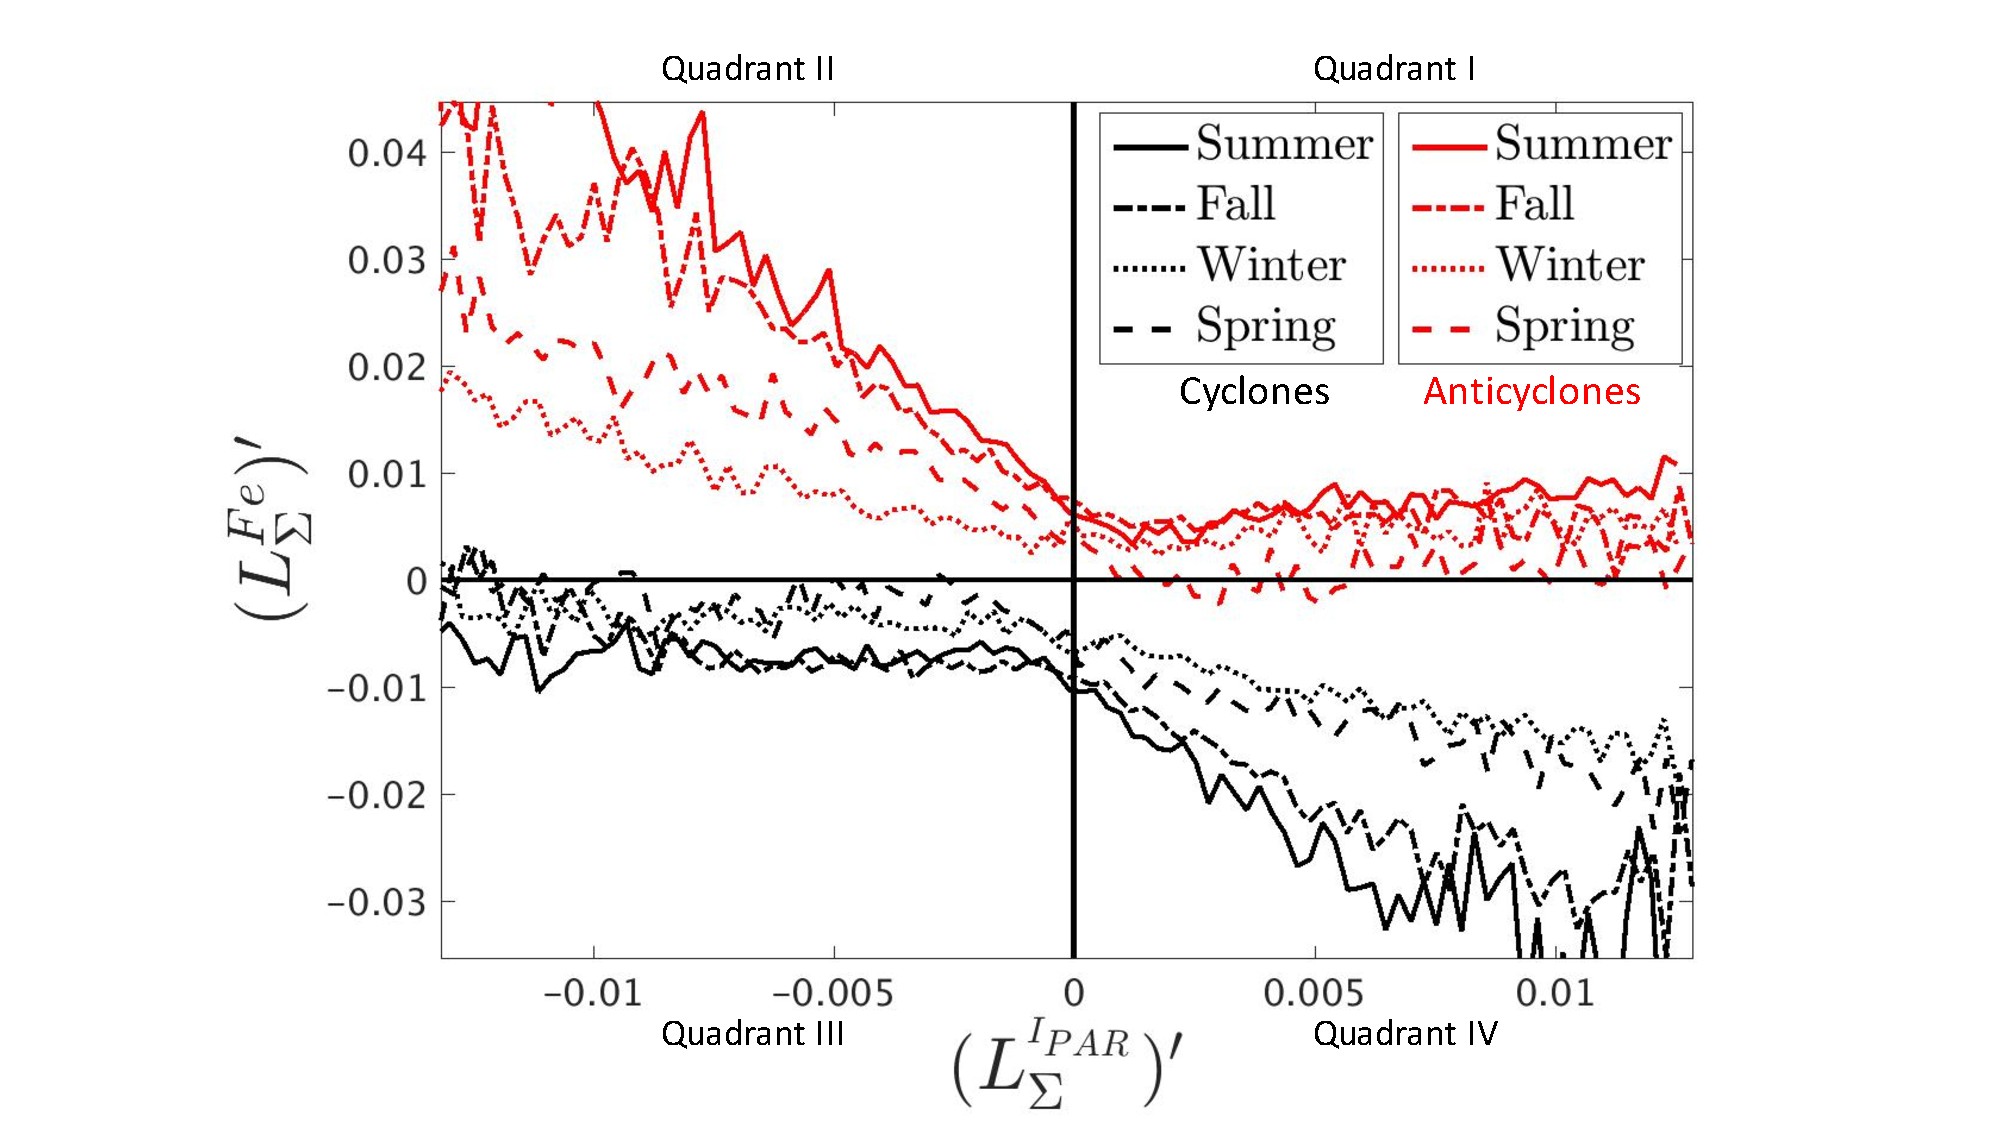
\includegraphics[scale=.6]{Fig11.pdf}
   \end{adjustwidth}
\caption[Seasonal variability in co-incident limitation terms. ]
{\textbf{Figure 10.} Seasonal variability in co-incident limitation terms. Community mean iron limitation ($L_\Sigma^{Fe}'$) is plotted as a function of the co-incident community mean light limitation ($L_\Sigma^{I_{PAR}}'$) for cyclones (black) and anticyclones (red). Eddies are seasonally binned into Summer (JFM, solid line), Fall (AMJ, dash/dot line), Winter (JAS, dotted line), and Spring (OND, dashed line). Note that more positive limitation terms correspond with less limitation. 
}
\label{fig:Fig10}
\end{figure}




%%%%%%%%% TABLES %%%%%%%%%%%%

%%%%%%%%%%%%%%%
%%  Table 1  %%
%%%%%%%%%%%%%%%
\definecolor{lightblue}{RGB}{153,205,255}
\definecolor{lightred}{RGB}{255,153,153}

\begin{table}[!htbp]
\begin{adjustwidth}{-1.2in}{-1.2in}
\renewcommand{\arraystretch}{2}
\centering


\begin{tabular}{ c | c || c || c | c ||  c | c ||c | c | c | c | c || c | c || c | c | }

\multicolumn{3}{c}{} & \multicolumn{6}{c}{\Huge{Cyclones}} & \multicolumn{1}{c}{} &  \multicolumn{6}{c}{\Huge{Antiyclones}}\\

\multicolumn{3}{c}{} & \multicolumn{6}{c}{\Large{Size}}& \multicolumn{1}{c}{}&
\multicolumn{6}{c}{\Large{Size}}\\

\hhline{~|~||~||-|-||-|-||-|-~-|-||-|-||-|-}

\multicolumn{3}{c|}{} &
\multicolumn{2}{|c||}{\large{Large}} & \multicolumn{2}{|c||}{\large{All}} & \multicolumn{2}{|c|}{\large{Small}} & &
\multicolumn{2}{|c||}{\large{Large}} & \multicolumn{2}{|c||}{\large{All}} & \multicolumn{2}{|c|}{\large{Small}}\\
\hhline{~:~::~::==::==::==~==::==::==}

\multicolumn{3}{c|}{} &
$freq$ & $mean$ & $freq$ & $mean$ & $freq$ & $mean$ & & $freq$ & $mean$ & $freq$ & $mean$ & $freq$ & $mean$ \\
\hhline{~:-::-::==::==::==~==::==::==}

\multirow{6}{1em}{\rotatebox{90}{\Large{Background Mixing}}}& \multirow{2}{1em}{\rotatebox{90}{\large{Deep}}} & $+ MLD'$ & \marktopleft{c1} \rowcolor{lightred} 19\% & 6m & 44\% & 14m & 58\% & 14m & \cellcolor{white} & 82\% & 30m & 67\%  & 22m & 56\% & 16m\\  

\hhline{~|~||-||-|-||-|-||-|-~-|-||-|-||-|-}

& & $- MLD'$ & \rowcolor{lightblue} 80\% & -32m \markbottomright{c1} & 56\% & -23m & 42\% & -18m & \cellcolor{white} & 18\% & -8m & 33\%  & -10m & 44\% & -12m  \\ 

\hhline{~:=::=::==::==::==~==::==::==}

& \multirow{2}{1em}{\rotatebox{90}{\large{All}}} & $+ MLD'$ & \rowcolor{lightred} 39\% &  3m & 50\% & 5m & 58\% & 6m & \cellcolor{white}& 60\% & 13m & 51\% & 8m & 43\% & 6m  \\ 

\hhline{~|~||-||-|-||-|-||-|-~-|-||-|-||-|-}

& & $- MLD'$ & \rowcolor{lightblue} 60\% & -13m & 50\%  & -8m & 42\% & -7m & \cellcolor{white} & 40\% & -4m & 49\%  & -5m & 57\% & -6m  \\ 

\hhline{~:=::=::==::==::==~==::==::==}
%%%%%%%%%
& \multirow{2}{1em}{\rotatebox{90}{\large{Shallow}}} & $+ MLD'$ & \rowcolor{lightred} 44\% & 3m & 51\% & 4m  & 58\% & 5m & \cellcolor{white}& 55\% & 6m & 47\% & 5m & 41\% & 4m  \\ 

\hhline{~|~||-||-|-||-|-||-|-~-|-||-|-||-|-}

& & $- MLD'$ & \rowcolor{lightblue} 55\% & -6m & 48\% & -5m & 42\% & -5m & \cellcolor{white} & 45\% & -3m & 53\%  & -4m & 58\% & -6m  \\ 
%%%%%%%%%
\hhline{~|-||-||-|-||-|-||-|-~-|-||-|-||-|-}

\end{tabular}
\end{adjustwidth}

\caption[Frequency and Magnitude of $MLD' (m)$.]
{\textbf{Table 1}. Frequency and Magnitude of $MLD' (m)$. The percent of cyclones (left table) and anticyclones (right table) with $+/- MLD'$ along with the mean magnitude of the anomaly for all qualifying eddies is denoted for nine subsets of eddies. Eddy subsets are delineated based on their size (Large: $L_S>50km$ \& $Amplitude>10cm$ | All: Unconstrained | Small: $L_S<50km$ \& $Amplitude < 10cm$) and the magnitude of background climatologic mixing (Deep: $MLD_{clim}>100m $ | All: Unconstrained | Shallow: $MLD_{clim}<100m $). For example, the cells enclosed by the dashed circle indicate that 25\% of large cyclones with deep $MLD_{clim}$ have a +$MLD'$ while 75\% have -$MLD'$. The mean value of qualifying eddies with +$MLD'$ is .10 $m$ and the mean value of qualifying eddies with -$MLD'$ is -29 $m$. $MLD'$ outliers in the top/bottom .5 percentile have been removed

$\sim$11,000 eddy large/deep mixing realizations }

\label{tab:Tab1}
\end{table}




%%%%%%%%%%%%%%%
%%  Table 2  %%
%%%%%%%%%%%%%%%
\definecolor{lightblue}{RGB}{153,205,255}
\definecolor{lightred}{RGB}{255,153,153}

\begin{table}[!htbp]
\begin{adjustwidth}{-1.2in}{-1.2in}
\renewcommand{\arraystretch}{2}
\centering


\begin{tabular}{ c | c || c || c | c ||  c | c ||c | c | c | c | c || c | c || c | c | }

\multicolumn{3}{c}{} & \multicolumn{6}{c}{\Huge{Cyclones}} & \multicolumn{1}{c}{} &  \multicolumn{6}{c}{\Huge{Antiyclones}}\\

\multicolumn{3}{c}{} & \multicolumn{6}{c}{\Large{Size}}& \multicolumn{1}{c}{}&
\multicolumn{6}{c}{\Large{Size}}\\

\hhline{~|~||~||-|-||-|-||-|-~-|-||-|-||-|-}

\multicolumn{3}{c|}{} &
\multicolumn{2}{|c||}{\large{Large}} & \multicolumn{2}{|c||}{\large{All}} & \multicolumn{2}{|c|}{\large{Small}} & &
\multicolumn{2}{|c||}{\large{Large}} & \multicolumn{2}{|c||}{\large{All}} & \multicolumn{2}{|c|}{\large{Small}}\\
\hhline{~:~::~::==::==::==~==::==::==}

\multicolumn{3}{c|}{} &
$freq$ & $mean$ & $freq$ & $mean$ & $freq$ & $mean$ & & $freq$ & $mean$ & $freq$ & $mean$ & $freq$ & $mean$ \\
\hhline{~:-::-::==::==::==~==::==::==}

\multirow{6}{1em}{\rotatebox{90}{\Large{Background Mixing}}}& \multirow{2}{1em}{\rotatebox{90}{\large{Deep}}} & $+ [Fe]'_\Sigma$ & \marktopleft{c1} \rowcolor{lightred} \% &  & \% &  & \% &  & \cellcolor{white} & \% &  & \%  &  & \% & \\  

\hhline{~|~||-||-|-||-|-||-|-~-|-||-|-||-|-}

& & $- [Fe]'_\Sigma$ & \rowcolor{lightblue} \% & - \markbottomright{c1} & \% &  & \% &  & \cellcolor{white} & \% &  & \%  &  & \% &   \\ 

\hhline{~:=::=::==::==::==~==::==::==}

& \multirow{2}{1em}{\rotatebox{90}{\large{All}}} & $+ [Fe]'_\Sigma$ & \rowcolor{lightred} \% &  & \% &  & \% & & \cellcolor{white}& \% & & \% &  & \% &   \\ 

\hhline{~|~||-||-|-||-|-||-|-~-|-||-|-||-|-}

& & $- [Fe]'_\Sigma$ & \rowcolor{lightblue} \% &  & \%  &  & \% &  & \cellcolor{white} & \% &  & \%  &  & \% &   \\ 

\hhline{~:=::=::==::==::==~==::==::==}
%%%%%%%%%
& \multirow{2}{1em}{\rotatebox{90}{\large{Shallow}}} & $+ [Fe]'_\Sigma$ & \rowcolor{lightred} \% &  & \% &  & \% &  & \cellcolor{white}& \% &  & \% &  & \% &   \\ 

\hhline{~|~||-||-|-||-|-||-|-~-|-||-|-||-|-}

& & $- [Fe]'_\Sigma$ & \rowcolor{lightblue} \% &  & \% &  & \% &  & \cellcolor{white} & \% &  & \%  &  & \% &   \\ 
%%%%%%%%%
\hhline{~|-||-||-|-||-|-||-|-~-|-||-|-||-|-}

\end{tabular}
\end{adjustwidth}

\caption[Frequency and Magnitude of $[Fe]'_\Sigma \; (mmol/m^{3})$.]
{\textbf{Table 2}. $[Fe]'_\Sigma \; (mmol/m^{3})$. Same as Table 1 for $[Fe]'_\Sigma$. Not that units ($mmol/m^{3}$) for mean anomalies are not included in table.}

\label{tab:Tab1}
\end{table}


%%%%%%%%%%%%%%%
%%  Table 3  %%
%%%%%%%%%%%%%%%
\definecolor{lightblue}{RGB}{153,205,255}
\definecolor{lightred}{RGB}{255,153,153}

\begin{table}[!htbp]
\begin{adjustwidth}{-1.2in}{-1.2in}
\renewcommand{\arraystretch}{2}
\centering


\begin{tabular}{ c | c || c || c | c ||  c | c ||c | c | c | c | c || c | c || c | c | }

\multicolumn{3}{c}{} & \multicolumn{6}{c}{\Huge{Cyclones}} & \multicolumn{1}{c}{} &  \multicolumn{6}{c}{\Huge{Antiyclones}}\\

\multicolumn{3}{c}{} & \multicolumn{6}{c}{\Large{Size}}& \multicolumn{1}{c}{}&
\multicolumn{6}{c}{\Large{Size}}\\

\hhline{~|~||~||-|-||-|-||-|-~-|-||-|-||-|-}

\multicolumn{3}{c|}{} &
\multicolumn{2}{|c||}{\large{Large}} & \multicolumn{2}{|c||}{\large{All}} & \multicolumn{2}{|c|}{\large{Small}} & &
\multicolumn{2}{|c||}{\large{Large}} & \multicolumn{2}{|c||}{\large{All}} & \multicolumn{2}{|c|}{\large{Small}}\\
\hhline{~:~::~::==::==::==~==::==::==}

\multicolumn{3}{c|}{} &
$freq$ & $mean$ & $freq$ & $mean$ & $freq$ & $mean$ & & $freq$ & $mean$ & $freq$ & $mean$ & $freq$ & $mean$ \\
\hhline{~:-::-::==::==::==~==::==::==}

\multirow{6}{1em}{\rotatebox{90}{\Large{Background Mixing}}}& \multirow{2}{1em}{\rotatebox{90}{\large{Deep}}} & $+ \mu'_\Sigma$ & \marktopleft{c1} \rowcolor{lightred} \% &  & \% &  & \% &  & \cellcolor{white} & \% &  & \%  &  & \% & \\  

\hhline{~|~||-||-|-||-|-||-|-~-|-||-|-||-|-}

& & $- \mu'_\Sigma$ & \rowcolor{lightblue} \% & - \markbottomright{c1} & \% &  & \% &  & \cellcolor{white} & \% &  & \%  &  & \% &   \\ 

\hhline{~:=::=::==::==::==~==::==::==}

& \multirow{2}{1em}{\rotatebox{90}{\large{All}}} & $+ \mu'_\Sigma$ & \rowcolor{lightred} \% &  & \% &  & \% & & \cellcolor{white}& \% & & \% &  & \% &   \\ 

\hhline{~|~||-||-|-||-|-||-|-~-|-||-|-||-|-}

& & $- \mu'_\Sigma$ & \rowcolor{lightblue} \% &  & \%  &  & \% &  & \cellcolor{white} & \% &  & \%  &  & \% &   \\ 

\hhline{~:=::=::==::==::==~==::==::==}
%%%%%%%%%
& \multirow{2}{1em}{\rotatebox{90}{\large{Shallow}}} & $+ \mu'_\Sigma$ & \rowcolor{lightred} \% &  & \% &  & \% &  & \cellcolor{white}& \% &  & \% &  & \% &   \\ 

\hhline{~|~||-||-|-||-|-||-|-~-|-||-|-||-|-}

& & $- \mu'_\Sigma$ & \rowcolor{lightblue} \% &  & \% &  & \% &  & \cellcolor{white} & \% &  & \%  &  & \% &   \\ 
%%%%%%%%%
\hhline{~|-||-||-|-||-|-||-|-~-|-||-|-||-|-}

\end{tabular}
\end{adjustwidth}

\caption[Frequency and Magnitude of $\mu'_\Sigma \; (mmol/m^{3})$.]
{\textbf{Table 3}. $\mu'_\Sigma \; (d^{-1})$. Same as Table 1 for $\mu'_\Sigma$. Not that units ($d^{-1}$) for mean anomalies are not included in table.}

\label{tab:Tab1}
\end{table}





%%%%%%%%%%%%%%%
%%  Table 5  %%
%%%%%%%%%%%%%%%

\definecolor{lightblue}{RGB}{153,205,255}
\definecolor{lightred}{RGB}{255,153,153}


\newcolumntype{b}{>{\columncolor{lightblue}}c}
\newcolumntype{r}{>{\columncolor{lightred}}c}


\begin{table}[!htbp]
\begin{adjustwidth}{-1.2in}{-1.2in}
\renewcommand{\arraystretch}{2}
\centering


\begin{tabular}{ c | c || c || r | b ||  r | b || r | b | c | r | b || r | b || r | b | }

\multicolumn{3}{c}{} & \multicolumn{6}{c}{\Huge{Cyclones}} & \multicolumn{1}{c}{} &  \multicolumn{6}{c}{\Huge{Antiyclones}}\\

\multicolumn{3}{c}{} & \multicolumn{6}{c}{\Large{Eddy Anomalies}}& \multicolumn{1}{c}{}&
\multicolumn{6}{c}{\Large{Eddy Anomnalies}}\\

\hhline{~|~||~||-|-||-|-||-|-~-|-||-|-||-|-}

\multicolumn{3}{c|}{} &
\multicolumn{2}{|c||}{\large{$\mu'_\Sigma \; (d^{-1})$}} & \multicolumn{2}{|c||}{\large{$MLD' \; (m)$}} & \multicolumn{2}{|c|}{\large{$[Fe'_\Sigma] \; (\frac{\mu mol}{m^3})$}} & &
\multicolumn{2}{|c||}{\large{$\mu'_\Sigma \; (d^{-1})$}} & \multicolumn{2}{|c||}{\large{$MLD' \; (m)$}} & \multicolumn{2}{|c|}{\large{$[Fe'_\Sigma] \; (\frac{\mu mol}{m^3})$}}\\
\hhline{~:~::~::==::==::==~==::==::==}

\multicolumn{3}{c|}{} &
\large{$+$} & \large{$-$} & \large{$+$} & \large{$-$} & \large{$+$} & \large{$-$} & & \large{$+$} & \large{$-$} & \large{$+$} & \large{$-$} & \large{$+$} & \large{$-$} \\
\hhline{~:-::-::==::==::==~==::==::==}

\multirow{9}{1em}{\rotatebox{90}{\Large{Subset}}}& \multirow{3}{1em}{\rotatebox{90}{\large{Large \& Deep}}} & $freq$ & \marktopleft{c1}  \% & \% & \% & \% & \% & \% & \cellcolor{white} & \% & \% & \%  &  \% & \% & \% \\  

\hhline{~|~||-||-|-||-|-||-|-~-|-||-|-||-|-}

& & $mean '$ &   & -  &  &  &  &  & \cellcolor{white} &  &  &   &  &  &   \\ 

\hhline{~|~||-||-|-||-|-||-|-~-|-||-|-||-|-}

& & $mean ''$ &  \% & - \markbottomright{c1} \% & \% & \% & \% & \% & \cellcolor{white} & \% & \% & \%  & \% & \% & \%  \\ 

\hhline{~:=::=::==::==::==~==::==::==}

& \multirow{3}{1em}{\rotatebox{90}{\large{All}}} & $freq$ &  \% & \% & \% & \% & \% & \% & \cellcolor{white} & \% & \% & \%  & \% & \% & \% \\  

\hhline{~|~||-||-|-||-|-||-|-~-|-||-|-||-|-}

& & $mean '$ &  &  &  &  &  &  & \cellcolor{white} &  &  &   &   &  &  \\  

\hhline{~|~||-||-|-||-|-||-|-~-|-||-|-||-|-}

& & $mean ''$ &  \% & \%  & \% & \% & \% & \% & \cellcolor{white} & \% & \% & \%  & \% & \% & \%  \\ 

\hhline{~:=::=::==::==::==~==::==::==}
%%%%%%%%%
& \multirow{3}{1em}{\rotatebox{90}{\large{Small \& Shallow}}} & $freq$ &  \% & \% & \% & \% & \% & \% & \cellcolor{white}& \% & \% & \% & \% & \% & \%  \\ 

\hhline{~|~||-||-|-||-|-||-|-~-|-||-|-||-|-}

& & $mean '$ &   &  &  &  &  &  & \cellcolor{white} &  &  &   &  &  &   \\ 
%%%%%%%%%

\hhline{~|~||-||-|-||-|-||-|-~-|-||-|-||-|-}


& & $mean ''$ &  \% & \%  & \% & \% & \% & \% & \cellcolor{white} & \% & \% & \%  & \% & \% &  \% \\ 

\hhline{~|-||-||-|-||-|-||-|-~-|-||-|-||-|-}

\end{tabular}
\end{adjustwidth}

\caption[Frequency and Magnitude of eddy anomalies.]
{\textbf{Table 5}. }

\label{tab:Tab1}
\end{table}
